% Created 2023-08-26 sam. 11:05
% Intended LaTeX compiler: pdflatex
\documentclass[a4paper,11pt]{book}



\usepackage[T1]{fontenc}
\usepackage{tgbonum}

\usepackage[lmargin=0.5in, rmargin=0.5in, paperwidth=29cm]{geometry}
\geometry{textwidth=23.1cm, textheight=24.50cm, marginratio={4:6,5:7}}


\usepackage{multicol}


\usepackage{framed,color,verbatim}

\usepackage[flushleft]{threeparttable}

\usepackage{minitoc}
\setcounter{minitocdepth}{5}


\usepackage{graphicx}
\usepackage{adjustbox}

\definecolor{shadecolor}{rgb}{.9, .9, .9}


\usepackage{fancyvrb}

\fvset{frame=single,framesep=1mm,fontfamily=courier,fontsize=\normalsize,numbers=left,framerule=.3mm,numbersep=1mm,commandchars=\\\{\}}

\usepackage[most]{tcolorbox}
\tcbset{
colback=gray!40,
colframe=white,
width=\dimexpr\textwidth\relax,
enlarge left by=0mm,
boxsep=5pt,
arc=0pt,outer arc=0pt,
}


\definecolor{applegreen}{rgb}{0.55, 0.71, 0.0}
\definecolor{antiquebrass}{rgb}{0.8, 0.58, 0.46}
\definecolor{PigBlue}{RGB}{14, 33, 160}
\definecolor{background}{rgb}{1.0, 0.96, 0.89}

\usepackage{listings}
\lstdefinestyle{coloredverbatim}{
backgroundcolor=\color{background!40}, % Background color
numbers=left,                    % Position of line numbers
numberstyle=\tiny\color{red!35!white},   % Style of line numbers
numbersep=5pt,                   % Space between code and line numbers
xleftmargin=18pt,                % Left margin
xrightmargin=-2pt,
frame=single,                    % Frame around the code
framexleftmargin=15pt,           % Left margin for the frame
framexrightmargin=5pt,           % Right margin for the frame
breaklines=true,                 % Allow line breaks
showstringspaces=false,          % Don't show spaces in strings
linewidth=0.95\linewidth,            % Fixed width size
basicstyle=\ttfamily\footnotesize, % Font style and size
captionpos=b,                     % Caption position
literate={π}{{$\pi$}}1,
language=C,
keywordstyle=[1]\color{purple},       % keyword style
morekeywords=[1]{let, copy, ref, dmut, mut, dcopy, is, def, unsafe, expand, alias}, % if you want to add more keywords to the set
keywordstyle=[2]\color{PigBlue!80},
keywords=[2]{i32, f32, i8, i16, i64, isize, u8, u16, u32, u64, usize, fsize, f32, f64, c8, c16, c32},
stringstyle = \color{black!30!applegreen}
}

\DeclareUnicodeCharacter{2320}{/}
\DeclareUnicodeCharacter{23AE}{|}
\DeclareUnicodeCharacter{2321}{/}
\DeclareUnicodeCharacter{2572}{\textbackslash}
\DeclareUnicodeCharacter{2571}{/}
\DeclareUnicodeCharacter{3C6}{$\phi$}
\DeclareUnicodeCharacter{2080}{${}_0$}
\DeclareUnicodeCharacter{3C0}{$\pi$}

\makeatletter
\renewcommand\tableofcontents{%
\@starttoc{toc}%
}
\makeatother


\usepackage{graphicx}
\usepackage{longtable}
\usepackage{wrapfig}
\usepackage{rotating}
\usepackage[normalem]{ulem}
\usepackage{amsmath}
\usepackage{amssymb}
\usepackage{capt-of}
\usepackage{hyperref}

\tikzstyle{every picture}+=[remember picture]
\tikzstyle{mProjectPP}=[circle,fill=yellow!70, minimum size=20pt,inner sep=0pt]
\tikzstyle{label}=[rectangle, fill=white, minimum size=40pt, inner sep=0pt]
\tikzstyle{Box}=[rectangle, fill=white, minimum size=40pt, inner sep=0pt]
\tikzstyle{Box2}=[rectangle, fill=white, minimum size=20pt, inner sep=0pt]


\usepackage{caption}
\usepackage{dblfloatfix}


\usepackage{makecell}


\setlength{\columnseprule}{0.01pt}
\def\columnseprulecolor{\color{black!10}}


\author{Emile Cadorel}
\date{\today}
\title{Ymir language specification 1.0}

\hypersetup{
  pdfauthor={Emile Cadorel},
  pdftitle={Ymir language specification 1.0},
  pdflang={English}}


\begin{document}
\setlength{\aweboxleftmargin}{0.05\linewidth}
\setlength{\aweboxcontentwidth}{0.93\linewidth}

%% \usepackage{utf8}
%% \setcode{utf8}

\maketitle
\dominitoc
\dominilof
\dominilot

\chapter*{Ymir releases}

Language specification of the Ymir language. This documentation is about the language specification, but is not a tutorial for the language.


The first stable release of Ymir is version 1.0, designed to be built using the
cxx\_version (version 0.1 of the Ymir compiler written in C++). Supporting tools
(such as GYC, Gyllir), the standard library and the documentation are released
with the same version number as the language release. GYC includes two versions:
the backend GCC version (e.g. 11.3.0) and the Ymir language version (e.g. 1.0).
The backend version should not affect the behaviour, only the frontend version
(ymirc version) has an effect.

\begin{multicols*}{2}
  \tableofcontents
\end{multicols*}


\chapter{Native scalar types}

This chapter dives into the semantic rules governing native types and their
behaviors. It outlines various operations like casting, binary and unary
operations, indexing, and more that can be performed on these types. The focus
here is on scalar types, while compound types will be discussed in the following
chapter. A scalar type inherently holds just one value and doesn't rely on or
borrow from other values. Consequently, it cannot be mutable on its own.
However, it can be part of a compound mutable type or a mutable variable,
allowing for mutability in broader context.

\begin{multicols*}{2}
  \minitoc%
  \section{Integers}
\label{sec:orga8b7d2e}

Integers are numbers without a decimal point. There are two types of integers,
signed and unsigned. The type of signed integers starts with the letter
\texttt{i}, while the type of unsigned integers starts with the letter
\texttt{u}.

\begin{center}
  \begin{tabular}{|r|ll|}
    \hline
    size & signed & unsigned\\[0pt]
    \hline
    \hline
    8 & \texttt{i8} & \texttt{u8}\\[0pt]
    16 & \texttt{i16} & \texttt{u16}\\[0pt]
    32 & \texttt{i32} & \texttt{u32}\\[0pt]
    64 & \texttt{i64} & \texttt{u64}\\[0pt]
    arch & \texttt{isize} & \texttt{usize}\\[0pt]
    \hline
  \end{tabular}
\end{center}

The size of the type in bits is written in the type itself, e.g. \texttt{i32} is
a signed int of 32 bits. The table above shows the list of integer types
implemented in version 1.0 of ymirc. \texttt{usize} and \texttt{isize} are
architecture dependent and have a size in bits that depends on the size of the
pointers on the target system, (i.e. 32 bits on 32 bit systems, 64 bits on 64
bit systems, and so on).


\vspace{-10pt}%
\subsection{Literals}
\label{sec:org2cf045d}

Integer literals can be written in four forms:
\begin{enumerate}
\item Octal, starting with \texttt{0o} and containing only numbers between \texttt{0} and \texttt{7}. (e.g. \texttt{0o71217}).
  \vspace{-2pt}%
\item Hexadecimal, starting with \texttt{0x} and containing numbers from
  \texttt{0} to \texttt{9} and letters from \texttt{a} to \texttt{f} in upper or
  lower case (e.g. \texttt{0xAB87fe}).
  \vspace{-2pt}%
\item Binary, starting with \texttt{0b} and containing numbers from \texttt{0} to
  \texttt{1} (e.g. \texttt{0b10010}).
  \vspace{-2pt}%
\item Decimal, starting with nothing special and containing numbers from
  \texttt{0} to \texttt{9} (e.g. \texttt{182993}).
\end{enumerate}

All four forms can also contain the token \texttt{\_} to separate long integer
literals and make them more readable (e.g. \texttt{1\_000\_000\_000\_000}).
There can be as many \texttt{\_} as you like, they will just be removed during
compilation.

Literals must end with a suffix to define a literal of an int type other than
\texttt{i32}. For example, to define a literal with value \texttt{67} and type
\texttt{i8}, you would write \texttt{67i8} or \texttt{0x43i8} or
\texttt{0o103i8}. A check is made during compilation to ensure that the selected
int type has enough bytes to encode the expected literal. Suffixes for
\texttt{isize} and \texttt{usize} are \texttt{is} and \texttt{us} respectively.

\subsection{Properties}
\label{sec:orgc02cb40}

Integer properties are accessed using the \texttt{::} operator (as for any type)
on a type expression. The properties are

\begin{center}
  \vspace{-3pt}
  \begin{adjustbox}{max width=\linewidth}
    \begin{tabular}{|l|ll|}
      \hline
      name & value & type\\[0pt]
      \hline
      \hline
      \texttt{init} & The initial value \texttt{0} & \texttt{typeof(x)}\\[0pt]
      \texttt{max} & The maximum value the type can encode & \texttt{typeof(x)}\\[0pt]
      \texttt{min} & The minimum value the type can encode & \texttt{typeof(x)}\\[0pt]
      \hline
      \texttt{typeid} & A string encoding the name of the type & \texttt{[c8]}\\[0pt]
      \hline
    \end{tabular}
  \end{adjustbox}
\end{center}

\smallskip

The following code shows an example of how type properties can be used.
\smallskip

\begin{lstlisting}[style=coloredverbatim]
  println (i32::max); // 2_147_483_647
  println (i16::min); // -32_768
\end{lstlisting}

\subsection{Casting}
\label{sec:orgfdc3d25}

Integer values can be cast to other types.

\begin{itemize}
\item To other integers: It is impossible to change the type of an int value
implicitly, i.e. it is impossible to transform a value of type \texttt{i32} into
a value of type \texttt{i64} without explicitly mentioning it. The cast operator
\texttt{cast!T (V)} can convert any int type to another int type.

There is one exception to the above rule. If a literal value is written without
a suffix, it can be cast to any int type as long as it is known at compile time.
An overflow check is performed to ensure that the casting is possible. For
example, the following is allowed.

  \begin{lstlisting}[style=coloredverbatim]
fn foo (a : u64) {
  // ...
}

let a : i64 = 1;
foo (7 + a); // 7 + a can be known at compilation time, 'a' is immutable and cte
  \end{lstlisting}

\item To char types: The cast operator can be used to convert an int type of
  type \texttt{u8} to a \texttt{c8}, a \texttt{u32} to a \texttt{c32} and a
  \texttt{u16} to a \texttt{c16} and vice versa (e.g. \texttt{c8} to
  \texttt{u8}). This is the only allowed casting from int to chars. Implicit
  casting is not allowed. The transformation does not change the value in any
  way (exactly the same bits before and after the cast).

  \begin{lstlisting}[style=coloredverbatim]
let a : c32 = cast!c32 (97u32);
let b : u8 = cast!u8 ('a'c8);
  \end{lstlisting}

\item To floating-point types: Casting to floating-point types is allowed from
  any int type whose type has a size of at least \texttt{4} bytes (\texttt{i32},
  \texttt{u32} and higher) to any floating-point type, and vice versa using the
  cast operator. This is the only allowed casting from int to float types.
  Implicit casting is not allowed. The value encoding is changed to be
  represented correctly. In fact, int and float have completely different ways
  of representing values in memory. The value is truncated when converted from a
  float to an int. And there may be some stepping when converting an int value
  to a float value, due to the holes in the set of values representable by the
  float encoding system.

  \begin{lstlisting}[style=coloredverbatim]
let a : f32 = cast!f32 (97u32);
let b : f64 = cast!f64 (12);

let c : i64 = cast!i64 (67.87);
  \end{lstlisting}

\end{itemize}

\subsection{Unary operators}
\label{sec:orge691bb5}

The following unary operators can be used on int types.
\smallskip


%% \begin{adjustbox}{max width=\linewidth}
\begin{center}
  \vspace{-5pt}
  \begin{threeparttable}
    \begin{tabular}{|l|ll|}
      \hline
      Operator & Operation & Example\\[0pt]
      \hline
      \hline
      \texttt{-} & Opposite value & \texttt{-19}\\[0pt]
      \hline
      \texttt{!} & Byte Not\(^{1}\) & \texttt{!19 == -20}\\[0pt]
      \hline
    \end{tabular}
    \begin{tablenotes}

    \item[1.] \footnotesize \textit{inverts each bit of the binary
      representation of the int value. This is semantically the same as
      computing \texttt{-x-1} (if the integer is signed).}

    \end{tablenotes}
  \end{threeparttable}
\end{center}
%% \end{adjustbox}

The result of unary operations always has the same type as the operand used in
the operation. The inverse operator \texttt{-} cannot be used on unsigned types
because they cannot be negative.


\subsection{Binary operators}
\label{sec:orgb91194f}

Binary operators with an int operand can only be used if both operands are of
type int. There are two exceptions to this rule: 1. When the operation involves
an object operand that has overridden the said binary operator (as a left or
right operand), 2. When one of the operands is of char or pointer type. Binary
operators involving char types are presented in the section on char types
(cf. Section~\ref{sec:char_type}), and those involving pointer types are presented in
the chapter on compound types (cf. Section~\ref{sec:pointer_type}).

The binary operators are divided into 5 groups:

\begin{itemize}
\item Arithmetics: Binary arithmetic operators can be used with two int values
  whose types have the same signed property (two signed operands or two unsigned
  operands, but not a mix). The result of the operation takes the type of the
  largest of the two operands, e.g. for an addition between a \texttt{i64} and a
  \texttt{i32} (e.g. \texttt{12 + 78i64}), the result takes the type
  \texttt{i64}. There is one exception, the exponent operator, where the right
  operand is always \texttt{i32} and the result is always of the type of the
  left operand.

  \begin{center}
    \vspace{-10pt}
    \begin{adjustbox}{max width=1.0\linewidth}
      \begin{tabular}{|c|lll|}
        \hline
        Operator & Operation & Commutative & Example\\[0pt]
        \hline
        \hline
        \texttt{+} & Addition & Yes & \texttt{1 + 2 == 3}\\[0pt]
        \texttt{-} & Subtraction & No & \texttt{2 - 1 == 1}\\[0pt]
        \texttt{*} & Multiplication & Yes & \texttt{3 * 4 == 12}\\[0pt]
        \texttt{/} & Division (truncate) & No & \texttt{13 / 3 == 4}\\[0pt]
        \texttt{\%} & Rest of the division & No & \texttt{13 \% 3 == 1}\\[0pt]
        \texttt{\textasciicircum{}\textasciicircum{}} & Exponant & No & \texttt{3\textasciicircum{}\textasciicircum{}4 == 81}\\[0pt]
        \hline
      \end{tabular}
    \end{adjustbox}
  \end{center}

\item Bytes: Bytes binary operators can be used with two int values of exactly
  the same type (e.g. \texttt{i64} with and only with \texttt{i64}).

  \begin{center}
    \vspace{-20pt}
    \begin{adjustbox}{max width=1.0\linewidth}
      \begin{tabular}{|c|l l l|}
        \hline
        Operator & Operation & Commutative & Example \\[0pt]
        \hline
        \hline
        \texttt{\(\vert\)} & Byte Or & Yes & \texttt{0b001} \(\vert{}\) \texttt{0b010 == 0b011}\\[0pt]
        \texttt{\&} & Byte And & Yes & \texttt{0b001 \& 0b010 == 0b000}\\[0pt]
        \texttt{\textasciicircum{}} & Byte Xor & Yes & \texttt{0b001 \textasciicircum{} 0b011 == 0b010}\\[0pt]
        \texttt{>>} & Byte left shift & No & \texttt{0b100000 >> 0b010 == 0b001000}\\[0pt]
        \texttt{<<} & Byte right shift & No & \texttt{0b001000 << 0b010 == 0b100000}\\[0pt]
        \hline
      \end{tabular}
    \end{adjustbox}
  \end{center}

\item Logical: Binary logical operators can be used with two integer values
  whose types have the same signed property (two signed operands or two unsigned
  operands, but not a mix). The largest type of the two integers is used to cast
  the value of the operand with the smallest type, to ensure that there is no
  overflow during the comparison. The result of the operation is always of type
  \texttt{bool}.

  \begin{center}
    \vspace{-20pt}
    \begin{adjustbox}{max width=1.0\linewidth}
      \begin{tabular}{|c|l l l|}
        \hline
        Operator & Operation & Commutative & Example\\[0pt]
        \hline
        \hline
        \texttt{>} & Greater than & No & \texttt{(12 > 11) == true}\\[0pt]
        \texttt{<} & Lower than & No & \texttt{(12 < 11) == false}\\[0pt]
        \texttt{>=} & Greater or equal & No & \texttt{(14 >= 14) == true}\\[0pt]
        \texttt{<=} & Lower or equal & No & \texttt{(11 <= 19) == true}\\[0pt]
        \texttt{==} & Equal & Yes & \texttt{(10 == 10) == true}\\[0pt]
        \texttt{!=} & Not equal & Yes & \texttt{(10 != 10) == false}\\[0pt]
        \hline
      \end{tabular}
    \end{adjustbox}
  \end{center}

\item Affectation: The affectation operator \texttt{=} can be used when the two
  operands are of exactly the same int type. The left operand must be a mutable
  lvalue (e.g. a mutable variable, a slice access, etc.). The affectation
  operator can be mixed with a math or byte operator (e.g. \texttt{+=},
  \texttt{\&=}, etc.). In this case, the operation \texttt{x += y} is rewritten
  as \texttt{x = x + (y)}, where the y operand always has a higher priority than
  the affectation operator. For example, the operation \texttt{x *= 12 + 3} is
  rewritten as \texttt{x = x * (12 + 3)}, even though the multiplication
  operator has a higher priority than the addition operator, i.e. the result of
  \texttt{x *= (12 + 3)} is different from the result of \texttt{x = (x * 12 +
    3)}.

  \begin{lstlisting}[style=coloredverbatim]
let mut a = 11;
let b = a * 12 + 3;
a *= 12 + 3;

assert (b == 135);
assert (a == 165);
  \end{lstlisting}

\item Range: The range operator can be used on int values of exactly the same
  type, creating a \texttt{range} value. The range type is a native compound
  type, described in the next chapter (cf. Section~\ref{sec:range_type}).

  \begin{center}
    \vspace{-10pt}
    \begin{adjustbox}{max width=1.0\linewidth}
      \begin{tabular}{|c|lll|}
        \hline
        Operator & Operation & Example & Interval\\[0pt]
        \hline
        \texttt{..} & Range operator not inclusive & \texttt{34 .. 12} & \texttt{[34;12[}\\[0pt]
            \texttt{...} & Range operator inclusive & \texttt{5 ... 89} & \texttt{[5;89]}\\[0pt]
            \hline
      \end{tabular}
    \end{adjustbox}
  \end{center}

The value of the result range has a default increment of \texttt{1} and its
inner type is the type of the operand. It can be ascending or descending
depending on the values used to construct it.

\end{itemize}

\subsection{Overflowing}
\label{sec:org0881da2}

Compile-time checks for value overflow are performed on \textit{cte} values.
There is no way to check for an overflow at runtime, and it may occur.

\begin{figure*}[t]
  \centering
  \scalebox{0.9}{
    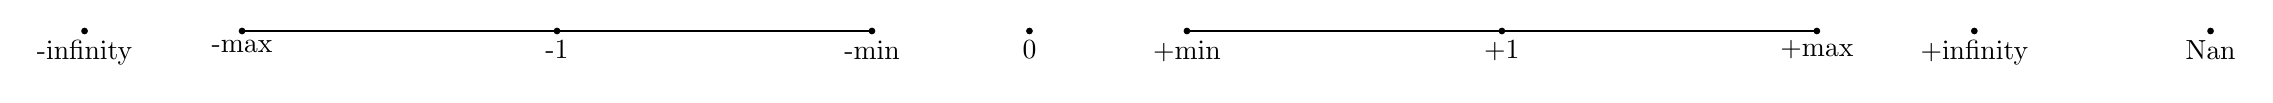
\begin{tikzpicture}
      \filldraw (0,0) circle (1pt) node[align=center, below] {-infinity};
      \filldraw (2,0) circle (1pt) node[align=center, below] {-max};
      \filldraw (6,0) circle (1pt) node[align=center, below] {-1};
      \filldraw (10,0) circle (1pt) node[align=center, below] {-min};
      \filldraw (12,0) circle (1pt) node[align=center, below] {0};
      \filldraw (14,0) circle (1pt) node[align=center, below] {+min};
      \filldraw (18,0) circle (1pt) node[align=center, below] {+1};
      \filldraw (22,0) circle (1pt) node[align=center, below] {+max};
      \filldraw (24,0) circle (1pt) node[align=center, below] {+infinity};
      \filldraw (27,0) circle (1pt) node[align=center, below] {Nan};

      \draw[-](2,0) -- (10, 0);
      \draw[-](14,0) -- (22, 0);

    \end{tikzpicture}
  }
  \caption{\label{float_point_size} Range of representable values with floating point types}
\end{figure*}


\section{Floating point types}
\label{sec:orgae6ed5f}

Floating point types refer to numbers with a floating decimal point. There are 4
floating point types, shown in the table below. The built-in floating point
types conform to IEEE 754 arithmetic, which means, for example, that
\texttt{f32} has 1 bit of sign, \texttt{8} bits of exponent, and \texttt{24} (23
explicit) bits of mantissa. The \texttt{fsize} type represents the largest
floating-point type that can be represented on the target architecture.

\begin{center}
  \vspace{-5pt}
  \begin{tabular}{|c|lll|}
    \hline
    type & size & exp & mantissa\\[0pt]
    \hline
    \hline
    \texttt{f32} & 32 & 8 & 24 (23 explicit)\\[0pt]
    \texttt{f64} & 64 & 11 & 53 (52 explicit)\\[0pt]
    \texttt{f80} & 80 & 16 & 64 (63 explicit)\\[0pt]
    \texttt{fsize} & arch & arch & arch\\[0pt]
    \hline
  \end{tabular}
\end{center}

\subsection{Literals}
\label{sec:orgfd9f825}

Floating point types can be written in three different forms, decimal,
scientific notation.

\begin{enumerate}
\item Decimal, two decimal int literals separated by the token \texttt{.} (with
  no spaces in between). \texttt{1837.0289}. The decimal part can be omitted,
  which means it is equal to \texttt{0} (e.g. \texttt{10.} is valid, but not
  \texttt{.10}).

\item Scientific notation, similar to decimal notation, but ending with an
  exponent preceded by the letter \texttt{e} or \texttt{E}. \texttt{3.14e78 ==
    (3.14 * 10.0 \textasciicircum{}\textasciicircum{} 78)}, which is \(3.14
  \times 10^{78}\). A sign for the exponential part can be set after the letter
  \texttt{e} or \texttt{E} with the token \texttt{-} or \texttt{+}, e.g.
  \texttt{3.e-10}. There must be no spaces in the literal.

\item Hexadecimal notation, starting with \texttt{0x}, then two hexadecimal int
  literal separated by the \texttt{.} token, followed by the letter \texttt{p}
  or \texttt{P}, and ending with a decimal int literal representing the
  exponential part. The fractional part can be empty, in which case the letter
  \texttt{p} follows the \texttt{.} token. However, the \texttt{.} token and the
  \texttt{p} exponential part are mandatory. A sign for the exponential part can
  be set after the letter \texttt{p} or \texttt{P} with the token \texttt{-} or
  \texttt{+}. There can be no spaces in the literal. Unlike scientific notation,
  the exponential part is a power of \texttt{2} instead of \texttt{10}, e.g.
  \texttt{0xA.p4 == (10.0 * 2.0\textasciicircum{}\textasciicircum{}4)}.

\end{enumerate}

The three forms can also contain the token \texttt{\_} to split long literals
and make them easier to read (e.g. \texttt{124\_732.789\_281},
\texttt{0x1.FFFF\_FFFFp1023}, \texttt{3.14\_15\_92e3f}). There can be as many
\texttt{\_} as you like, they will just be removed during compilation. Literals
can end with a suffix to specify the type of the literal; \texttt{f} to define
\texttt{f32} literals, \texttt{d} to define \texttt{f64} (for \texttt{double}),
\texttt{l} for \texttt{f80} (for \texttt{long}) and \texttt{r} for
\texttt{fsize} (for \texttt{real}). Literals without a suffix are considered to
be of type \texttt{f64}. The literals \texttt{4.5e10f} and \texttt{0.8f},
\texttt{0x1.FFp10f} are of type \texttt{f32} and \texttt{4.5e10} and
\texttt{0.8}, \texttt{0x1.FFp10} are of type \texttt{f64}.

\subsection{Properties}
\label{sec:org52a5d6e}

Floating point properties can be accessed by using the \texttt{::} operator on a
type expression. The properties are as follows:

\begin{center}
  \vspace{-5pt}
  \begin{adjustbox}{max width=1.01\linewidth}
    \begin{threeparttable}
      \begin{tabular}{|l|ll|}
        \hline
        Name & Meaning & Type\\[0pt]
        \hline
        \hline
        \texttt{init} & The initial value - nan (Not a Number) & \texttt{typeof(x)}\\[0pt]
        \Xhline{0.001pt}
        \texttt{max} & The maximal finite value & \texttt{typeof(x)}\\
        & that this type can encode & \\[0pt]
        \Xhline{0.001pt}

        \texttt{min} & The minimal finite value & \texttt{typeof(x)}\\
        & that this type can encode & \\[0pt]
        \Xhline{0.001pt}

        \texttt{nan} & The value Not a Number & \texttt{typeof(x)}\\[0pt]
        \Xhline{0.001pt}
        \texttt{inf} & The value positive infinity & \texttt{typeof(x)}\\[0pt]
        \Xhline{0.001pt}
        \texttt{epsilon} & The smallest increment & \texttt{typeof(x)}\\
        & to the value 1 &\\[0pt]
        \Xhline{0.001pt}
        \texttt{dig} & The number of decimal digit of precision & \texttt{u32}\\[0pt]
        \Xhline{0.001pt}
        \texttt{mant\_dig} & Number of bits in the mantissa & \texttt{u32}\\[0pt]
        \Xhline{0.001pt}
        \texttt{max\_10\_exp} & The maximum value &  \texttt{i32} \\
        & such that \(10^{max\_10\_exp}\) is representable &\\[0pt]
        \Xhline{0.001pt}
        \texttt{max\_exp} & The maximum value & \texttt{i32}\\
        & such that \(2^{max\_exp-1}\) is representable & \\[0pt]
        \Xhline{0.001pt}
        \texttt{min\_10\_exp} & The minimum value & \texttt{i32}\\
        & such that \(10^{min\_10\_exp}\) is representable$^1$  & \\[0pt]
        \Xhline{0.001pt}
        \texttt{min\_exp} & The minimum value & \texttt{i32}\\
        & such that \(2^{min\_exp-1}\) is representable$^1$ & \\[0pt]
        \hline
        \texttt{typeid} & A string encoding the name of the type & \texttt{[c8]}\\[0pt]
        \hline
      \end{tabular}
      \begin{tablenotes}
      \item[1.] \small \textit{as a normalized value}
      \end{tablenotes}
    \end{threeparttable}
  \end{adjustbox}
\end{center}

\smallskip

The \texttt{min} value is not the opposite of the \texttt{max} value. The
figure~\ref{float_point_size} describes the ordering relationship between values
of floating-point types, where points and lines are the values that can be
represented by a floating-point type.

\subsection{Casting}
\label{sec:org9eacb07}

Floating point values can be cast to other types.

\begin{itemize}
\item To other floating-point types: It is impossible to change the type of a
  float implicitly. The cast operator \texttt{cast!T (V)} can convert any float
  value to another float value of another float type. Because float values of
  different float types are coded with different numbers of bits, there may be
  stepping during casting.

\item To integer types: The cast operator can be used to convert a float value
  of any float type to an int value whose type is at least 4 bytes in size
  (\texttt{i32}, \texttt{u32} and larger). If the cast operator is used, the
  value is truncated to the floor value (e.g. \texttt{1.3} \texttt{1.5} and
  \texttt{1.8} are all truncated to \texttt{1}), and anything that was part of
  the decimal part of the float is lost. The reverse cast is also allowed (from
  any int type whose size is at least \texttt{4} bytes to any float type); in
  this case, some stepping may occur due to the floating-point encoding.

\end{itemize}

Floating point values cannot be converted to other types.

\subsection{Unary operators}
\label{sec:org30770bf}

The \texttt{-} unary operators can be used on floating point types. The result
of the operation is the opposite value and is of the same type as the operand of
the operation. For example, \texttt{-89.0f} is of type \texttt{f32}.

\subsection{Binary operators}
\label{sec:orga43d13a}

Binary operators involving a float operand can only be used if both operands are
floats. There is an exception to this rule when the operation involves an object
operand that has overridden the said binary operator (as a left or right
operand). The binary operators are divided into 4 groups:

\begin{itemize}
\item Arithmetic: Binary arithmetic operators can be used with two float values.
  The result of the operation takes the type of the largest operand (e.g. an
  operation with \texttt{f32} and \texttt{f64} takes the type \texttt{f64}). The
  operators that can be used are described in the table below.

  \begin{center}
    \vspace{-20pt}
    \begin{adjustbox}{max width=1.0\linewidth}
      \begin{tabular}{|c|lll|}
        \hline
        Operator & Operation & Commutative & Example\\[0pt]
        \hline
        \hline
        \texttt{+} & Addition & Yes & \texttt{1.0 + 2.3 == 3.3}\\[0pt]
        \texttt{-} & Subtraction & No & \texttt{1. - 8. == -7.}\\[0pt]
        \texttt{*} & Multiplication & Yes & \texttt{3. * 4. == 12.}\\[0pt]
        \texttt{/} & Division & No & \texttt{7. / 3. == 2.333}\\[0pt]
        \texttt{\%} & Rest of division & No & \texttt{7.23 \% 3.09 == 1.05}\\[0pt]
        \texttt{\textasciicircum{}\textasciicircum{}} & Exponant & No & \texttt{7. \textasciicircum{}\textasciicircum{} 3 == 343.}\\[0pt]
        \hline
      \end{tabular}
    \end{adjustbox}
  \end{center}

  The power operator \texttt{\textasciicircum{}\textasciicircum{}} is a special
  operator that can take a float or an integer as its right operand. If both
  operands are floats, then they must be of exactly the same type, and the
  result value takes the type of the operands. If the right operand is an int
  value, then the result of the operation takes the type of the left operand.

\item Logical: Binary logical operators can be used with two float values. The
  largest type of the two operands is used to cast the value of the operand with
  the smallest type, to avoid too much stepping (although stepping may still
  occur). The result of the operation is always of type \texttt{bool}.

  \begin{center}
    \vspace{-20pt}
    \begin{adjustbox}{max width=1.0\linewidth}
      \begin{tabular}{|c|lll|}
        \hline
        Operator & Operation & Commutative & Example\\[0pt]
        \hline
        \hline
        \texttt{>} & Greater than & No & \texttt{(12. > 11.) == true}\\[0pt]
        \texttt{<} & Lower than & No & \texttt{(12. < 11.) == false}\\[0pt]
        \texttt{>=} & Greater or equal & No & \texttt{(14. >= 14.) == true}\\[0pt]
        \texttt{<=} & Lower or equal & No & \texttt{(11. <= 19.) == true}\\[0pt]
        \texttt{==} & Equal & Yes & \texttt{(10. == 10.) == true}\\[0pt]
        \texttt{!=} & Not equal & Yes & \texttt{(10. != 10.) == false}\\[0pt]
        \texttt{<=>} & Is congruent & Yes & \texttt{(10. <=> 10.) == true}\\[0pt]
        \texttt{<!>} & Is not congruent & Yes & \texttt{(10. <!> 10.) == false}\\[0pt]
        \hline
      \end{tabular}
    \end{adjustbox}
  \end{center}

   \texttt{<=>} and \texttt{<!>} are special floating point operators designed
   to evaluate the equality and inequality of left and right operands, taking
   into account the possibility of stepping. In other words, it uses the
   \texttt{::epsilon} value of the floating point type (of the largest operand)
   to evaluate whether the left operand is equal to the right operand delta the
   epsilon value. They also check for \texttt{nan} equality and inequality.
   These operators are of course less efficient than the equality and inequality
   operators, as they involve multiple instructions and possibly conditional
   jumps.

\item Affectation: The affectation operator \texttt{=} can be used when the two
  operands are of exactly the same float type. The left operand must be a
  mutable lvalue (e.g. a mutable variable, a slice access, etc.). The
  affectation operator can be mixed with an arithmetic operator (e.g.
  \texttt{+=}, \texttt{/=}, etc.). In this case, the operation \texttt{x += y}
  is rewritten as \texttt{x = x + (y)}, where the y operand always has a higher
  priority than the affectation operator. For example, the operation \texttt{x
    *= 12. + 3.} is rewritten as \texttt{x = x * (12. + 3.)}, even though the
  multiplication operator has a higher priority than the addition operator, i.e.
  the result of \texttt{x *= (12. + 3.)} is different from the result of
  \texttt{x = (x * 12. + 3.)}.

  \begin{lstlisting}[style=coloredverbatim]
let mut a = 11.0;
let b = a * 12.0 + 3.0;
a *= 12.0 + 3.0;

assert (b == 135.0);
assert (a == 165.0);
  \end{lstlisting}

\item Range: The range operator can be used on two float values of exactly the
  same type, creating a \texttt{range} value. The range type is a native
  compound type, which is described in the following chapter (see
  section~\ref{sec:range_type}).

  \begin{center}
    \vspace{-20pt}
    \begin{adjustbox}{max width=1.0\linewidth}
      \begin{tabular}{|l|lll|}
        \hline
        Operator & Operation & Example & Interval\\[0pt]
        \hline
        \hline
        \texttt{..} & Range operator not inclusive & \texttt{34.f .. 12.f} & \texttt{[34.f;12.f[}\\[0pt]
            \texttt{...} & Range operator inclusive & \texttt{5.f ... 89.f} & \texttt{[5.f;89.f]}\\[0pt]
            \hline
      \end{tabular}
    \end{adjustbox}
  \end{center}


  The value of the result range has a default increment of \texttt{1.0} and its
  inner type is the type of the operand. It can be ascending or descending
  depending on the values used to construct it.

\end{itemize}

\subsection{Overflowing and stepping}
\label{sec:orgd5d9f51}

Because of the way float values are encoded, there are gaps in the set of values
they can represent. Thus, some operations that should be mathematically
equivalent do not always produce the same float value. To compare two float
values, the property \texttt{::epsilon} can be used, as well as the congruent
operators \texttt{<=>} and \texttt{<!>}. There is no value overflow checking
at compile time or runtime.

\section{Bool}
\label{sec:org9f3a743}

The Bool type is a simple type, whose name is \texttt{bool}, and that can only
describe two values \texttt{true} and \texttt{false}. It is stored in a single
byte of memory, although only the first bit is used and has meaning.

\subsection{Properties}
\label{sec:org503bc9e}

Properties of the type \texttt{bool} are accessible by using the operator
\texttt{::} on a type expression. The properties are as follows:

\begin{center}
  \vspace{-5pt}
  \begin{adjustbox}{max width=\linewidth}
    \begin{tabular}{|l|ll|}
      \hline
      Name & Meaning & Type\\[0pt]
      \hline
      \hline
      \texttt{init} & The initial value \texttt{false} & \texttt{bool}\\[0pt]
      \hline
      \texttt{typeid} & A string encoding the name of the type & \texttt{[c8]}\\[0pt]
      \hline
    \end{tabular}
  \end{adjustbox}
\end{center}

\subsection{Literals}
\label{sec:org7620b9c}

Boolean literals are the keywords \texttt{true} and \texttt{false}.

\subsection{Casting}
\label{sec:org7cd1f94}

A value of type \texttt{bool} can be cast to a value of type \texttt{u8} using
the cast operator, in which case the value \texttt{false} is converted to the
value \texttt{0u8} and the value \texttt{true} is converted to the value
\texttt{1u8}. The reverse conversion is impossible using the cast operator, but
can be carried out using the equality operators of type int (e.g. \texttt{1u8 ==
  1u8}). This is the only cast allowed for the boolean type. It is impossible to
convert a boolean value to a value of another type without explicitly using the
cast operator.

\subsection{Unary operators}
\label{sec:orgb412ce4}

The unary operator \texttt{!} can be used on a boolean value to get its opposite
value (i.e. \texttt{!true} becomes \texttt{false} and \texttt{!false} becomes
\texttt{true}).

\subsection{Binary operators}
\label{sec:org030ae50}

Binary operators involving a bool operand can only be used if both operands are
of type bool. There is an exception to this rule when the operation involves an
object operand that has overridden the said operator (as a left or right
operand).

Binary operators are divided into 3 groups:

\begin{itemize}
\item Affectation: Affectation operators can be used to change the value of a
  mutable lvalue of type bool using a right operand of type bool. Because there
  are no arithmetic operators that can be used on a bool value, no arithmetic
  operator can be attached to the affectation operation. \texttt{\&\&=} and
  \texttt{||=} are not valid operators, and their use results in a syntax error.

\item Comparisons: The comparison operators \texttt{==} and \texttt{!=} can be
  used with two bool values to evaluate equality and inequality respectively.
  The result of the operations is always of type \texttt{bool}. By convention,
  it is not recommended to use equality and inequality operators to test the
  \texttt{bool} values. In fact, \texttt{a == false} can be rewritten as
  \texttt{!a}, and \texttt{a == true} is simply \texttt{a}.

\item Logical: Logical operators can be used with two bool operands.

  \begin{center}
    \vspace{-20pt}
    \begin{adjustbox}{max width=1.0\linewidth}
      \begin{tabular}{|c|l l l|}
        \hline
        Operator & Operation & Commutative & Example\\[0pt]
        \hline
        \hline
        \texttt{\(\vert\vert\)} & Or & No & \texttt{false} \(\vert{} \vert{}\) \texttt{true == true}\\[0pt]
        \texttt{\&\&} & And & No & \texttt{true \&\& false == false}\\[0pt]
        \hline
      \end{tabular}
    \end{adjustbox}
  \end{center}

  The operators \texttt{\&\&} and \texttt{||} are marked as non-commutative. This
  is not because they can return a different value if the left and right operands
  are inverted, but because for \texttt{\&\&} the right operand is not evaluated
  if the left operand is false, and for \texttt{||} the right operand is not
  evaluated if the left operand is true. This can be useful when chaining tests.

  \begin{lstlisting}[style=coloredverbatim]
let i = 12;
let p = &i;

// if 'p is null', '*p == 12' is not evaluated
let a = p !is null && *p == 12;

// if 'p is null', '*p != 12' is not evaluated
let b = p is null || *p != 12;

// foo function is not called
let c = true || foo ();

// foo function is called
let d = false || foo ();
  \end{lstlisting}
\end{itemize}

\section{Characters}
\label{sec:char_type}

Character types are used to encode characters (ASCII or Unicode). There are
three character types \texttt{c8}, \texttt{c16} and \texttt{c32} with a size of
\texttt{8}, \texttt{16} and \texttt{32} bits respectively. These char types are
encoding values in utf-8, utf-16 and utf-32.

\begin{center}
  \vspace{-5pt}
  \begin{tabular}{ll}
    Value & Content\\[0pt]
    \hline
    \texttt{\textbackslash{}a} & Alert beep, (Bell)\\[0pt]
    \texttt{\textbackslash{}b} & Backspace\\[0pt]
    \texttt{\textbackslash{}f} & Page break\\[0pt]
    \texttt{\textbackslash{}n} & New line\\[0pt]
    \texttt{\textbackslash{}r} & Carriage return\\[0pt]
    \texttt{\textbackslash{}t} & Horizontal tab\\[0pt]
    \texttt{\textbackslash{}v} & Vertical tab\\[0pt]
    \texttt{\textbackslash{}\textbackslash{}} & Backslash\\[0pt]
    \texttt{\textbackslash{}'} & Apostrophe\\[0pt]
    \texttt{\textbackslash{}"} & Double quotation mark\\[0pt]
    \texttt{\textbackslash{}u\{\}} & Unicode\\[0pt]
  \end{tabular}
  \captionof{table}{\label{tab:escape_chars} Escape characters}
\end{center}

\subsection{Properties}
\label{sec:orgf9fbc31}

The properties of char types can be accessed by using the \texttt{::} operator
on a type expression. The properties are as follows:

\begin{center}
  \vspace{-5pt}
  \begin{adjustbox}{max width=\linewidth}
    \begin{tabular}{|l|ll|}
      \hline
      Name & Meaning & Type\\[0pt]
      \hline
      \hline
      \texttt{init} & The initial value \texttt{\textbackslash{}u\{0\}} & \texttt{typeof(x)}\\[0pt]
      \hline
      \texttt{typeid} & A string encoding the name of the type & \texttt{[c8]}\\[0pt]
      \hline
    \end{tabular}
  \end{adjustbox}
\end{center}


\subsection{Literals}
\label{sec:org73c4919}

Char literals are enclosed by the token \texttt{'} and can be described using three forms:

\begin{enumerate}
\item Using the direct representation of the character (e.g. \texttt{π}),
\item Using an escape character. The escape chars are described in the
  table~\ref{tab:escape_chars}.

\item Using an int literal representation of Unicode. To avoid confusing the int
  literal representation with the literal of the int itself, the int literal
  must be encoded using the escape character \texttt{\textbackslash{}u} and the
  tokens \texttt{\{} and \texttt{\}}. For example
  \texttt{\textbackslash{}u\{0x263A\}}, \texttt{\textbackslash{}u\{0b1101\}} or
  \texttt{\textbackslash{}u\{10\}}.

\end{enumerate}

As with float or int literals, a suffix must be added at the end of the literal
to define the value with the correct type. For example, to define a \texttt{c8}
value containing the character \texttt{a}, write \texttt{'a'c8}. Literal values
without a suffix are considered to be of type \texttt{c32}.

\begin{lstlisting}[style=coloredverbatim]
let a : c32 = 'r';
let b : c8 = '\u{10}'c8;
let d = 'π';
let e = '\n'c8;

assert (e == b);
\end{lstlisting}

\subsection{Casting}
\label{sec:org16d703f}

Char types can be cast using the cast operator. It is not possible to implicitly convert a char value to a value of another type.

\begin{itemize}
\item To other char types: The cast operator can be used to convert a char of
  one size to a char of another size. This does not guarantee encoding validity.
  The standard library defines more complex transformations that respect
  encoding in the \texttt{std::conv} module.

\item To integer types: The cast operator can be used to transform a char value
  of type \texttt{c8} into a \texttt{u8}, a \texttt{c16} into a \texttt{u16} and
  a \texttt{c32} into a \texttt{u32}. The transformation does not change the
  value in any way (exactly the same bits before and after the cast).

\end{itemize}

\subsection{Unary operators}
\label{sec:org78546fb}

No unary operators can be used on char types.

\subsection{Binary operators}
\label{sec:orge863f7d}

Binary operators on character types are divided into four groups.

\begin{itemize}
\item Arithmetic: Binary arithmetic operators can be used with a char value and
  an unsigned int value (of the same size, e.g. for \texttt{c8} and
  \texttt{u8}). The result always takes the type of the char operand. It is
  impossible to add or subtract two char values, even if they are of exactly the
  same type.

  \begin{center}
    \vspace{-5pt}\begin{adjustbox}{max width=1.0\linewidth}
      \begin{tabular}{|c|lll|}
        \hline
        Operator & Operation & Commutative & Example\\[0pt]
        \hline
        \hline
        \texttt{+} & Addition & Yes & \texttt{'a' + 16u32 == 'q'}\\[0pt]
        \texttt{-} & Subtraction & No & \texttt{'q' - 16u32 == 'a'}\\[0pt]
        \hline
      \end{tabular}
  \end{adjustbox}\end{center}


  Char values can be used as right operands in arithmetic operations. The type of
  the result operation would still be the type of the char operand, and the int
  operand would still have to be of the same size as the char operand, so
  \texttt{('q' + 12u32) == (12u32 + 'q')}.

\item Logical: Binary logical operators can be used with two char values of
  exactly the same type. The result of the operation is always of type
  \texttt{bool}.

  \begin{center}
    \vspace{-10pt}\begin{adjustbox}{max width=1.0\linewidth}
      \begin{tabular}{|c|lll|}
        \hline
        Operator & Operation & Commutative & Example\\[0pt]
        \hline
        \hline
        \texttt{>} & Greater than & No & \texttt{('q' > 'a') == true}\\[0pt]
        \texttt{<} & Lower than & No & \texttt{('q' < 'a') == false}\\[0pt]
        \texttt{>=} & Greater or equal & No & \texttt{('q' >= 'q') == true}\\[0pt]
        \texttt{<=} & Lower or equal & No & \texttt{('b' <= 'r') == true}\\[0pt]
        \texttt{==} & Equal & Yes & \texttt{('a' == 'a') == true}\\[0pt]
        \texttt{!=} & Not equal & Yes & \texttt{('a' != 'a') == false}\\[0pt]
        \hline
      \end{tabular}
  \end{adjustbox}\end{center}

\item Affectation: The affectation operator \texttt{=} is usable when the left
  operand is a mutable lvalue and the right operand is strictly the same char
  type as the left operand.

  The affectation operator can be mixed with an arithmetic operator \texttt{+=}
  and \texttt{-=}, in which case the right operand must be a value whose type is
  an unsigned int with a size exactly equal to the size of the char type of the
  left operand. The affectation \texttt{x += y} is rewritten as \texttt{x = x +
    (y)}, where the y operand always has a higher priority than the affectation
  operator.

  \begin{lstlisting}[style=coloredverbatim]
let mut a = 'a';

let b = a + 21u32;

a = 'e';
a += 7u32;

assert (b == 'v');
assert (a == 'l')
  \end{lstlisting}

\item Range: The range operator can be used on two char values whose types are
  strictly identical, creating a range value.

  \begin{center}
    \vspace{-10pt}\begin{adjustbox}{max width=1.0\linewidth}
      \begin{tabular}{|l|lll|}
        \hline
        Operator & Operation & Example & Interval\\[0pt]
        \hline
        \hline
        \texttt{..} & Range operator not inclusive & \texttt{'a' .. 'z'} & \texttt{[a;z[}\\[0pt]
            \texttt{...} & Range operator inclusive & \texttt{'a' ... 'r'} & \texttt{[a;r]}\\[0pt]
            \hline
      \end{tabular}
  \end{adjustbox}\end{center}


  The result value has a default increment of \texttt{1} and its inner type is
  the type of the operands. It can be increasing or decreasing depending on the
  values used to construct it.

\end{itemize}

\subsection{Overflowing}
\label{sec:orga9c18c5}

Compile time overflow checking is done on \textit{cte} values. The check ensures
that the chosen type is large enough to encode the value. There is no way to
check for overflow at runtime, and it can happen. It is also possible, due to
the encoding, that a value is not a valid unicode or ascii value if it is
created at runtime (e.g. \texttt{'π' + 501u32}).

\section{Void}
\label{sec:org409c2d8}

The \texttt{void} type is a special type that has no value and occupies
\texttt{0} byte of memory. Unlike other types, it cannot be used to declare
variables. There is no literal to describe a void type, as it cannot take a
value. There is no way to cast a void type to another type, there is no value to
transform. For the same reason, there are no operators applicable to void types.

\vspace{-10pt}
\subsection{Properties}
\label{sec:orgffa98ee}

The properties of a void type can be accessed by using the \texttt{::} operator
on a type expression. The properties are:

\begin{center}
  \vspace{-5pt}
  \begin{adjustbox}{max width=\linewidth}
    \begin{tabular}{|l|ll|}
      \hline
      Name & Meaning & Type\\[0pt]
      \hline
      \hline
      \texttt{typeid} & A string encoding the name of the type & \texttt{[c8]}\\[0pt]
      \hline
    \end{tabular}
  \end{adjustbox}
\end{center}

\end{multicols*}

\chapter{Native compound types}
\label{chap:compound}

This chapter presents the semantic specification of native compound types and
their associated behaviour. It lists the casting, binary, unary, index\ldots
operators and other permitted operations on the types presented. This chapter
also discusses the mutability of compound types, as they often contain borrowed
values. Some \texttt{pragma} operations are applicable to compound types, but
they are not covered in this chapter; a specific chapter on \texttt{pragma}
operators is presented in the Chapter~\ref{chap:conditional_compilation}.

\begin{multicols*}{2}
  \minitoc%
%% \end{multicols*}%
%% \begin{multicols*}{2}
  \section{Preamble}%
\label{sec:preamble_compound_types}

Before presenting the specifications of the different compound types, let's
define some useful language elements.


\begin{itemize}
\item \textit{Data borrowing} -- A data borrowing value is a value that points
  to data that is not automatically copied when the value is copied. The
  simplest example of data borrowing is the use of a pointer type, where the
  value of the pointer provides information about a memory address containing
  data. The data that the pointer points to is not copied when the pointer is
  copied. An illustration of this is given in figure~\ref{fig:data_borrowing}.
  In this example, both variables \texttt{x} and \texttt{y} borrow the data
  located on the heap at address \texttt{0xfa45b987}. Copying the value of the
  variable \texttt{y} to another variable does not make a copy of the borrowed
  value (which is on the heap), but only copies the value directly inside
  \texttt{y}, which in this case is on the stack. The borrowed data can be on
  the stack or on the heap, and the same can be said for the borrowing data.
  Such memory is called "borrowed" because it can live longer than the value
  pointing to it, and the pointer only temporarily borrows its value for reading
  or writing.

  In the case of borrowing data, mutability is crucial because multiple variables
  refer to the same segment of memory. This can lead to unpredictable side
  effects. Memory mutability is used to manage such behaviour and to ensure that
  only a few variables have mutable access to values. Most importantly, it is a
  safeguard against the accidental creation of mutable memory references.


\end{itemize}
\begin{figure}[H]
  \centering
  \begin{adjustbox}{max size=\linewidth}
    \begin{tikzpicture}
      % ================ Axis ========================
      \draw (0, 0) -- coordinate (LEFT) (0, 0);
      \draw[-Stealth](0, 10) -- coordinate (YAx) (0, 1.5);
      \draw[-Stealth](7.2, 10) -- coordinate (YAx) (7.2, 1.5);
      \draw[Box] (3.5, 10.7) -- (3.5, 10.7) node[anchor=center]{\textbf{STACK}};

      \filldraw (0, 6.5) circle (1pt) node[align=center, left] {+0};
      \filldraw (0, 5.5) circle (1pt) node[align=center, left] {+8};
      \filldraw (0, 4.5) circle (1pt) node[align=center, left] {+16};
      \filldraw (0, 3.5) circle (1pt) node[align=center, left] {+24};
      \filldraw (0, 2.5) circle (1pt) node[align=center, left] {+32};

      %% % ================ Foo ========================
      \fill[black!10] (0.2, 10) rectangle (7, 8);
      \draw[Box] (3.5, 7.6) -- (3.5, 7.6) node[anchor=center]{\textbf{.}};
      \draw[Box] (3.5, 7.4) -- (3.5, 7.4) node[anchor=center]{\textbf{.}};
      \draw[Box] (3.5, 7.2) -- (3.5, 7.2) node[anchor=center]{\textbf{.}};

      \draw[line width=1pt] (0.18, 6.9) rectangle (7.02, 2.48);
      \fill[olive!10] (0.2, 6.5) rectangle (7, 2.5);
      \draw[Box] (3.5, 6.7) -- (3.5, 6.7) node[anchor=center]{\emph{foo}};

      \draw[Box] (0.5, 5.5) -- (0.5, 5.5) node[anchor=center]{\textbf{\textit{x}}};
      \draw[line width=0.005pt] (0.3, 6.4) rectangle (6.8, 4.6);
      \draw[line width=0.005pt] (0.7, 5.5) rectangle (6.8, 5.5);

      \draw[Box] (3.5, 6) -- (3.5, 6) node[anchor=center]{\emph{len~=}~$3$};
      \draw[Box] (3.5, 5) -- (3.5, 5) node[anchor=center]{\emph{ptr~=}~0xfa45b987};

      \draw[Box] (0.5, 3.5) -- (0.5, 3.5) node[anchor=center]{\textbf{\textit{y}}};
      \draw[line width=0.005pt] (0.3, 4.4) rectangle (6.8, 2.6);
      \draw[line width=0.005pt] (0.7, 3.5) rectangle (6.8, 3.5);

      \draw[Box] (3.5, 4) -- (3.5, 4) node[anchor=center]{\emph{len~=}~$3$};
      \draw[Box] (3.5, 3) -- (3.5, 3) node[anchor=center]{\emph{ptr~=}~0xfa45b987};


      %% % ================ Heap ========================

      \draw[-Stealth](10, 10) -- coordinate (YAx) (10, 1.5);
      \draw[-Stealth](17.2, 10) -- coordinate (YAx) (17.2, 1.5);
      \filldraw (17.2, 7.5) circle (1pt) node[align=center, right] {0xfa45b987};

      % ================ Data ========================
      \draw[Box] (13.5, 10.7) -- (13.5, 10.7) node[anchor=center]{\textbf{HEAP}};
      \fill[black!10] (10.2, 10) rectangle (17, 8);
      \fill[teal!20] (10.2, 7.9) rectangle (17, 5);
      \draw[line width=0.005pt] (10.4, 7) rectangle (16.8, 7);
      \draw[line width=0.005pt] (10.4, 6) rectangle (16.8, 6);

      \draw[Box] (13.5, 7.5)  (13.8, 7.5) node[anchor=center]{$1$};
      \draw[Box] (13.5, 6.5)  (13.8, 6.5) node[anchor=center]{$2$};
      \draw[Box] (13.5, 5.5)  (13.8, 5.5) node[anchor=center]{$3$};

      \draw[thick,-Stealth,shorten >=1pt] (7.3, 5) to [out=0,in=180] node[below left, yshift=3mm] {} (9.9, 7.5);

      \draw[thick,-Stealth,shorten >=1pt] (7.3, 3) to [out=0,in=180] node[below left, yshift=3mm] {} (9.9, 7.5);

    \end{tikzpicture}
  \end{adjustbox}
  \vspace{-30pt}%
  \caption{\label{fig:data_borrowing}Example of data borrowing}
\end{figure}
%
%% \vspace{2pt}%

\begin{itemize}
\item \textit{Data movement} -- Data movement is the process of copying a value
  from one segment of memory to another. This can be done by allocation, memory
  copy (or deep copy), function calls and other operations. Data movements are
  always explicit, which ensures that no unwanted copies are made that could
  potentially slow down the program.

\item \textit{lvalue} -- An lvalue refers to the left operand in a \textit{data
  movement} operation. In other words, it is an expression that refers to a
  segment of memory that is modified as a result of the \textit{data movement}.
  An lvalue can take various forms, including a simple variable, a function
  parameter, an index operation, and more.

\item \textit{rvalue} -- An rvalue is the right operand involved in a
  \textit{data movement} operation. A rvalue can be aliased (using the keyword
  \texttt{alias}), referenced (keyword \texttt{ref}), copied with
  (\texttt{copy}, \texttt{dcopy}), or it can be implicit. Implicit means that
  the \textit{data movement} does not borrow mutable data and can therefore be
  allowed implicitly. In the case of an implicit \textit{data movement} there is
  no copying of borrowed data and there is no new borrowing of mutable memory.

\end{itemize}

\section{Pointers}%
\label{sec:pointer_type}

Pointers are values storing an address of memory. Pointer types are described
using the \texttt{*} token followed by a type (e.g. \texttt{*i32} describing a
pointer to a \texttt{i32} value). In the beta version of Ymir (compiler written
in c++) the operator \texttt{\&} was used, it was changed as it was also used to
refer to object instances that are in a way pointers but have very different
behavior.

\subsection {Literals}

The keyword \texttt{null} is used to describe a pointer pointing to nowhere.
This is the only literal that can be used as a pointer value.

\subsection {Construction}

To construct a pointer, the unary operator \texttt{\&} can be used on a lvalue
(for example, a variable). This operator returns the address of the value
referenced by the operand, i.e. \texttt{\&a} returns the address of the segment
of memory referenced by the variable \texttt{a}. For the sake of simplicity, we
can say that we are retrieving the address of the variable \texttt{a}.

\begin{lstlisting}[style=coloredverbatim]
let a = 12;
let b : *i32 = &a;
\end{lstlisting}

\subsection {Mutability}

Because pointers borrow data from another value (value pointed by the pointer),
their mutability is important. A pointer has two level of mutability:
\begin{enumerate}
\item \texttt{mut *T}, In this case, the pointer can be changed, but the value
  inside the pointer cannot be changed.
\item \texttt{mut *(mut T)}, In this case, both the value to which the pointer
  is pointing and the pointer itself can be changed.
\end{enumerate}

A mutable pointer (\textit{level 1}) means that if the pointer is contained
inside another compound type or variable, then the value it points to can be
changed. Checking for mutability is done at compile time when borrowing a value
to construct a pointer value.

\begin{lstlisting}[style=coloredverbatim]
let dmut a : *i32 = null;

let b = 12;
a = &b; // not allowed 'b' is not mutable
*a = 24; // but it would be modified by this operation


let mut c = 11;
a = &c; // allowed c is mutable
*a = 24; // modify the value of c is allowed
\end{lstlisting}

The keyword \texttt{alias} must be used on the right operand when data borrowing
is transferred to the left operand. In practice, this means that if the
mutability of the left operand is second level (i.e. \texttt{mut *(mut T)}), the
keyword \texttt{alias} must be used, and the right operand must also be second
level mutable. The keyword can be omitted if the aliasing is obvious (i.e. by
function return, or construction such as the unary operator \texttt{\&}).

\subsection {Properties}

Pointer type properties can be accessed using the \texttt{::} operator on a type
expression. The properties are as follows: following:

% \vspace{-20pt}%
\begin{center}\begin{adjustbox}{max width=\linewidth}
  \begin{tabular}{|l|ll|}
    \hline
    Name & Meaning & Type\\
    \hline
    \hline
    \texttt{init} & The initial value \texttt{null} & \texttt{typeof(x)}\\
    \hline
    \texttt{typeid} & A string encoding the name of the type & \texttt{[c8]} \\
    \hline
  \end{tabular}
\end{adjustbox}\end{center}

\subsection {Casting}

A pointer type can be cast to any pointer type using the cast operator
\texttt{cast!T(V)}. A pointer is a really low-level type with few guarantees,
but some operations rely on this possibility to perform generic operations
(common trait \texttt{Packable} for example). The mutability of the result is
the same as the mutability of the operand, if the value is explicitely aliased,
it is immutable otherwise. This is the only allowed cast on pointer types.

\begin{lstlisting}[style=coloredverbatim]
  let dmut a : [i32]  = copy [12];
  let dmut b : *[i32] = &a;

  // c : dmut *[f32];
  let dmut c = cast!{*[f32]} (alias b);

  // not allowed, from *[f32] to dmut *[f32];
  let dmut d = cast!{*[f32]} (b);
\end{lstlisting}

\subsection {Unary operators}

The unary operator \texttt{*} is used on a pointer value to dereference it and
access the value pointed to by the pointer. This operation is unsafe and may
cause the program to crash. If the operation does not crash, it does not
necessarily mean that the pointer was created correctly. This operation is
unsafe and can only be used in a \texttt{unsafe} context.

\begin{lstlisting}[style=coloredverbatim]
let i = 10;
let x = &i;

unsafe {
  let j = *x;
}
\end{lstlisting}

\subsection {Binary operators}

Binary operators are divided into 3 groups:
\begin{itemize}
\item Arithmetic: Pointer arithmetic is allowed with a \texttt{usize} as the
  right operand. Unlike the C language, the arithmetic does not depend on the
  size of the data pointed to by the pointer. The operation adds a number of
  bytes to the address, which means that the addition operation with a left
  operand whose value is \texttt{0xabc0} and a right operand \texttt{8us} will
  always have the value \texttt{0xabc8}, regardless of the type of content
  pointed to by the pointer. The behaviour is not the same with the index
  operator. The type of the result of the operation is always the same as the
  type of the left operand.

  %
  %\vspace{-14pt}%
  \begin{center}\begin{adjustbox}{max width=1\linewidth}
    \begin{tabular}{|c|lll|}
      \hline
      Operator & Operation & Commutative & Example \\
      \hline
      \hline
      \texttt{+} & Addition & Yes & \texttt{\&a + 2us} \\
      \texttt{-} & Substraction & No & \texttt{\&a - 2us} \\
      \hline
    \end{tabular}
  \end{adjustbox}\end{center}

\item Logical: Comparison operators always return a value of type \texttt{bool}
  and can only be used if the two operands are of the same pointer type (e.g.
  \texttt{*i32} with \texttt{*i32}).

  \vspace{-10pt}%
  \begin{center}\begin{adjustbox}{max width=1\linewidth}
      \begin{threeparttable}
        \begin{tabular}{|c|lll|}
          \hline
          Operator & Operation & Commutative & Example \\
          \hline
          \hline
          \texttt{==} & Equality test & Yes & \texttt{(\&a == \&a) == true}\\
          \texttt{!=} & Inequality test & Yes & \texttt{(\&a != \&a) == false}\\
          \texttt{<} & Lower than & No & \texttt{(\&a < \&a + 1us) == false}\\
          \texttt{>} & Greater than & No & \texttt{(\&a > \&a - 1us) == true}\\
          \texttt{>=} & Greater or equal$^{1^{\phantom{j}}}$ & No & \texttt{(\&a >= \&a - 1us) == true}\\
          \texttt{<=} & Lower or equal$^{1^{\phantom{j}}}$ & No & \texttt{(\&a <= \&a - 1us) == false}\\
          \hline
        \end{tabular}
    \end{threeparttable}
    \end{adjustbox}\end{center}

\item Affectation: The affectation operators are usable when the two operands
  are of exactly the same pointer type. The mutability level of the left operand
  must be less than or equal to the mutability level of the right operand.
  Affection operators can be mixed with arithmetic operators (e.g. \texttt{+=},
  \texttt{-=}). In this case the operation is rewritten as \texttt{x = x + y}
  and \texttt{y} must be a value of type \texttt{usize}.

  \begin{lstlisting}[style=coloredverbatim]
let mut a = 11;
let dmut b = &a;

let mut c = &a;
b = c; // not allowed it will discard the const property
c = b; // No problem the mutability level of c is lower than the one of b

c += 1us;

let dmut d = &a;
b = alias d; // alias is needed, data is borrowed
  \end{lstlisting}

\end{itemize}

\subsection {Index operator}

The index operator can be used on a pointer left operand with an int value as
the index right operand. The result of the operation is the dereferencing of the
pointer value by the offset of the value used as index. Unlike pointer
arithmetic using the \texttt{+} and \texttt{-} operators, the index operator
takes into account the size of the data pointed to by the pointer, i.e. the
index operation \texttt{(\&a)[7]} is strictly transformed into \texttt{*(\&a +
  (7us * sizeof (\_\_pragma!inner (typeof(\&a), 0)))}. This operation is unsafe because it
dereferences a raw pointer.

\smallskip

\begin{lstlisting}[style=coloredverbatim]
let mut a = 12;
let dmut b = &a;

unsafe {
  b [0] = 89;
}
assert (a == 89);
\end{lstlisting}

\smallskip

The mutability of the result value depends on the mutability level of the
pointer operand. If the mutability level of the pointer operand is 2, then the
result can be used as lvalue.

\section {Tuples}


Tuples are anonymous structures that store a set of data of different types.
They are described as a list of types enclosed in parentheses (e.g.
\texttt{(i32, f32, c8)}). A tuple may have only one inner type, in which case
the token \texttt{,} is added after the definition of the inner type (e.g.
\texttt{(i32,)}).

\subsection {Literals}

Tuple literals are described as a list of values enclosed in parentheses, for
example \texttt{(1, 'r', false)} is a tuple literal whose type is \texttt{(i32,
  c32, bool)}. Tuples containing only one value must have the token \texttt{,}
after the declaration of the value to distinguish them from priority operations
enclosed in parentheses.

\begin{lstlisting}[style=coloredverbatim]
let a = (1, 'r', false);
let b : (i32,) = (23,); // tuple value
let c : i32 = (23); // int value
\end{lstlisting}

\noindent Tuple inner values are constructed in the order in which they are
written. In the following example, the function \texttt{foo} is called before
the function \texttt{bar}.

\begin{lstlisting}[style=coloredverbatim]
fn foo ()-> i32 {
  println ("In foo.");
  12
}

fn bar ()-> f32 {
  println ("In bar.");
  34.0f
}

let a = (foo (), bar ());
\end{lstlisting}

\subsection {Mutability and memory alignment}%
\label{sec:tuple_mutability}

The mutability of tuple values cannot be described as a level of mutability, as
might be the case for other compound types. In the case of tuples, mutability is
defined as a tree, where each node of the tree depends on the mutability of its
parent. For example, the mutability of the following tuple type \texttt{mut (mut
  i32, f32, dmut *c8)} is shown in the figure~\ref{fig:tuple_mutability}.

\begin{figure}[H]
  \centering
  \scalebox{1.3}{
    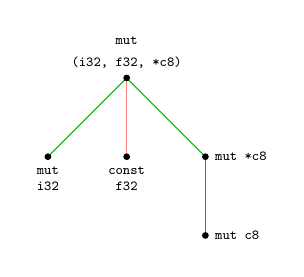
\begin{tikzpicture}

      \draw[-, black!30!green] (0,0) -- (-1,-1);
      \draw[-, red!50] (0,0) -- (0,-1);
      \draw[-, black!30!green] (0,0) -- (1,-1);
      \draw[-, black!30!green] (1,-1) -- (1,-2);

      \filldraw (0, 0.3) node[align=center, above] {\texttt{\tiny{mut}}};
      \filldraw (0, 0) circle (1pt) node[align=center, above] {\texttt{\tiny{(i32, f32, *c8)}}};
      \filldraw (-1,-1) circle (1pt) node[align=center, below]{\texttt{\tiny{mut}}};
      \filldraw (-1,-1.2) node[align=center, below]{\texttt{\tiny{i32}}};
      \filldraw (0,-1) circle (1pt) node[align=center, below]{\texttt{\tiny{const}}};
      \filldraw (0,-1.2) node[align=center, below]{\texttt{\tiny{f32}}};
      \filldraw (1,-1) circle (1pt) node[align=center, right]{\texttt{\tiny{mut *c8}}};
      \filldraw (1,-2) circle (1pt) node[align=center, right]{\texttt{\tiny{mut c8}}};


    \end{tikzpicture}
  }
  \caption{\label{fig:tuple_mutability} Example of tuple mutability}
\end{figure}


The mutability level of inner types is only important when they are borrowing
data. In the previous example shown in figure~\ref{fig:tuple_mutability}, only
the mutability of the inner type \texttt{*c8} is important during data movement.
In other words, a value of type \texttt{mut (i32, f32, dmut *c8)} can be passed
to it without any problem. As with any borrowing type, the keyword
\texttt{alias} must be used when borrowing data.

\begin{lstlisting}[style=coloredverbatim]
let mut x = 't'c8;
let mut a : mut (mut i32, f32, dmut *c8) = (1, 12.0f, &x);
let mut b : mut (i32, f32, dmut *c8) = (1, 7.0f, null);

a = alias b; // no problem
b = alias a; // no problem either

let c : (i32, f32, *c8) = (1, 7.0f, &x);
a = alias c; // not allowed, it would dicard constant property of the third field
\end{lstlisting}

Tuple types with mutable values that don't borrow data are considered
non-borrowing types, and therefore don't need \texttt{alias} during data
movement. In practice, all the data of such a tuple is copied during data
movement.

The alignment of tuples follows the same rules as the alignment of structures
(see chapter~\ref{chap:structures}), basically they are just anonymous
structures.

\subsection {Properties}

Pointer type properties can be accessed by using the \texttt{::} operator on a
type expression. The properties are as follows:
\smallskip

\begin{center}
  \begin{adjustbox}{max width=\linewidth}
    \begin{tabular}{|l|ll|}
      \hline
      Name & Meaning & Type\\
      \hline
      \hline
      \texttt{init} & The inital value of the tuple & \texttt{usize} \\
      & where every inner field are set to \texttt{T::init} & \\
      \Xhline{0.001pt}
      \texttt{arity} & The number of inner elements of the tuple type & \texttt{usize}\\
      \hline
      \texttt{init} & A string encoding the name of the type & \texttt{[c8]} \\
      \hline
    \end{tabular}
  \end{adjustbox}
\end{center}

\smallskip

Inner types are not accessible using the \texttt{::} operator, but are
accessible using \texttt{\_\_pragma}. Pragmas are presented in the
section~\ref{sec:pragmas}.

\subsection {Binary operators}

Binary operators are divided into 3 groups:
\begin{itemize}
\item Access: The operator \texttt{.} is used to access a given field of the
  tuple. The right operand must be of type int and must be within the range of
  \texttt{0} and the arity of the tuple to be accessed. The result of the
  operation takes the type of the field at the index described by the right
  operand, and so does the value. The first field index is \texttt{0}.

  \begin{lstlisting}[style=coloredverbatim, linewidth=0.95\linewidth]
let mut a : (mut i32, f32) = (8, 8.f);

a._0 = 7; // allowed first field is mutable
a._1 = 1.f; // not allowed, second field is not mutable

let c = a.(12 - 11); // accessing the field at index 1
  \end{lstlisting}

\item Comparison: The comparison operators \texttt{==} and \texttt{!=} are
  defined on tuples when each of the inner types are comparable. It compares all
  fields of two tuples and checks whether all inner values are equal for
  \texttt{==} or at least one inner value is different between the two operands
  for the operator \texttt{!=}.

  There is no relation of order between the tuples, even if they are of the same
  type, since in general such a comparison would be meaningless.

\item Affectation: The affectation operator creates a \textit{data movement}
  from the right operand to the left operand. Mutability must be respected when
  data is borrowed. Data mutability on tuples has already been introduced in
  section~\ref{sec:tuple_mutability}.

\end{itemize}

\subsection {Dollar operator}

The dollar operator can be used within an access binary operation in the right
operand expression. The dollar value takes the value of the arity of the tuple,
and its type is \texttt{usize}. Its value is known at compile time.

\begin{lstlisting}[style=coloredverbatim]
let a = (1, 9.0f, 'r');

let b = a.($ - 1us); // access the last value, i.e. 'r'
\end{lstlisting}

\subsection {Tuple expansion}

Tuples have a special operator called \texttt{expand} that turns them into a
list of parameters. Expanding a tuple is useful to create other tuples, or to
pass the data of the tuple as function parameters.

\begin{lstlisting}[style=coloredverbatim]
fn foo (a : i32, b : f32) {}

let a = (1, 5.f);

 // transform a into a list of values
let b : (i32, f32, c32) = (expand a, 't');

foo (expand a); // transform a into a list of parameters
\end{lstlisting}

Such an operation is done at compile time and is simply a rewrite that is less
verbose. In fact, in the previous example, the line \texttt{foo (expand a)} is
rewritten as \texttt{foo (a.0, a.1)}. The mutability level of the expanded
values is always \texttt{1}, which means that tuple expansion can never borrow
mutable data. Tuple expansions are useful in variadic template functions to
write generic operations on a list of variadic parameters.

\subsection {Tuple deconstruction}

Tuple can be used to declare several variables at once, using the same
\texttt{let} declaration. We call this declaration a tuple deconstruction
because it splits the values of the tuple into a list of variables. Types of
variables inside tuple deconstruction can be specified the same way they would
be specified for normal variable declaration. This can be used to define more
complex levels of mutability.

\begin{lstlisting}[style=coloredverbatim]
  // a is mutable, but not b nor c
let (mut a, b, c) = (1, 't', 12.f);

assert (a == 1 && b == 't' && c == 12.f);

// With type specifications
let (mut d : i32, mut e : [mut f32 ; 2]) = (1, [1.f, 2.f]);
\end{lstlisting}

A variadic variable can be used as the last variable declaration in such a
deconstruction with the token \texttt{...}. In this case, it's type is always a
tuple that takes all the values in the tuple that are left and not associated
with other variables. The type of this last variable can be specified before the
token \texttt{...}.

\begin{lstlisting}[style=coloredverbatim]
let (a, b...) = (1, 2, 3);

assert (a == 1);
assert (b == (2, 3));

let (c, d...) = (1, 2);

assert (c == 1);
assert (d == (2,));

// With type specifications
let (e, f : (i32, f32)...) = (1, 2, 3.f);
\end{lstlisting}

The mutability level of variables declared using tuple deconstruction can be
mutable by using the keywords \texttt{mut} or \texttt{dmut} on specific
variables of the tuple deconstruction (i.e. \texttt{let (dmut a, b) = alias
  t;}). In that case the right operand must match the mutability, and be aliased
explicitly.


\subsection {Tuple iteration}

Tuples are iterable types, so they can be used as the iterable value of a
\texttt{for} loop. In practice, because such an iteration would create iterator
variables of different types, the iteration is unrolled at compile time. The
tuple value is only constructed once before entering any loop body.

\begin{lstlisting}[style=coloredverbatim]
let a = (1, 't', 89.0f);
for i in a {
    println (i);
}

// would be rewritten into
println (a._0);
println (a._1);
println (a._2);
\end{lstlisting}

Two variables can be used as iterators, the first being the index of the
iteration and the second being the value within the tuple. If only one variable
is defined, only the value of the tuple fields is contained in the iterator.
Iterators are always immutable and never used as references, but this limitation
can easily be circumvented by using the index iterator to access the tuple.

\begin{lstlisting}[style=coloredverbatim]
let dmut a = (1, 2, 3);
for i, _ in a {
    a.(i) = 9;
}

assert (a == (9, 9, 9));
\end{lstlisting}

More information about \texttt{for} loops is presented in Section~\ref{sec:for_loops}.

\section {Ranges}%
\label{sec:range_type}

Range is a compound type consisting of four elements that describe a range of
values. The four elements are \texttt{fst} the first value of the range (e.g.
\texttt{0}), \texttt{scd} the last value of the range (e.g. \texttt{10}),
\texttt{step} the step of the range (e.g. \texttt{2}), and \texttt{contains} of
type bool, which indicates whether the last value \texttt{scd} is contained in
the range or not. There are only three types that can describe the inner
components of a range: integer, floating point and character. The type of the
range is defined by the inner type followed by the token \texttt{..} (e.g.
\texttt{i32..} describes a range of \texttt{i32} values). Range are useful for
iteration or for accessing a subset of values (for example, a subset of a
slice).

\subsection {Literals}

Range literals are described using the \texttt{..} token or the \texttt{...}
token. The \texttt{..} token is used to define a range whose final value is not
included in the range, and the \texttt{...} token defines a range whose final
value is included. If different tokens are used to describe the literal, the
type is the same, and the \texttt{..} token is always the only token used to
describe a range type.

\begin{lstlisting}[style=coloredverbatim]
let a : i32.. = 0 .. 2;
let b : i32.. = 0 ... 2;

assert (a.fst == b.fst);
assert (a.scd == b.scd);
assert (a.step == b.step);
assert (!a.contains && b.contains);
\end{lstlisting}

Range values can be decreasing, in which case the step is negative. Note that
for ranges of unsigned integers and character values, it is theoretically
impossible to have a negative value for the step. However, there is a bit of
cheating going on here, using the overflow limitation of types to create a value
that, when added to \texttt{fst}, equals \texttt{fst - abs (step)} (in practice,
this is exactly the same as adding a negative value at the binary level, but it
is not really the valid high level representation). For this reason it can be
considered that step is always a signed version of the type, even if the field
type is considered to be the same as the type of the inner values (\texttt{fst}
and \texttt{scd}), and thus one bit of its encoding is always used for the sign.

The \texttt{fst} value of the range literal is constructed before the
\texttt{scd} value. In the following example, the function \texttt{foo} is
called before the function \texttt{bar}.

\begin{lstlisting}[style=coloredverbatim]
fn foo ()-> i32 {
  println ("In foo.");
  12
}

fn bar ()-> i32 {
  println ("In bar.");
  1
}

let a = (foo ()) .. (bar ());
\end{lstlisting}

\subsection {Mutability and memory alignement}

As expected, range values do not share any data, and every field included in the
value is replicated during data movement. Therefore, there is no concern for
mutability, rendering the type not aliasable. A mutable range has the ability to
modify its internal fields, but even if the range type is a compound type, it
operates precisely like a scalar type since it can never contain any borrowed
data. In memory a range value has the same memory alignement as the structure
(cf. Chapter~\ref{chap:structures}) presented in the following source code where
\texttt{T} is the inner type of the range.

\begin{lstlisting}[style=coloredverbatim]
struct {T}
| fst : T
| scd : T
| step : T
| contains : bool
-> Range;
\end{lstlisting}

\subsection {Properties}

Range type properties can be accessed through the operator \texttt{::} applied
to a type expression. The following properties include:

\begin{center}\begin{adjustbox}{max width=\linewidth}
  \begin{tabular}{|l|ll|}
    \hline
    Name & Meaning & Type\\
    \hline
    \hline
    \texttt{init} & The initial value ranging from \texttt{T::init} & \texttt{typeof (x)}\\
    & to \texttt{T::init} with a step of \texttt{T::init} and & \\
    & with contains set to \texttt{false} where \texttt{T} is & \\
    & the inner type (e.g. \texttt{i32} for \texttt{i32..}). &\\
    \hline
    \texttt{typeid} & A string encoding the name of the type & \texttt{[c8]} \\
    \hline
  \end{tabular}
\end{adjustbox}\end{center}


\subsection {Binary operators}

Binary operators are divided into 4 groups:

\begin{itemize}
\item Access: The operator \texttt{.} is utilized to access the field of the
  range type. The right operand is the name of the field to access. The fields
  are listed in the table below.

  %\vspace{-20pt}%
  \begin{center}\begin{adjustbox}{max width=\linewidth}
    \begin{threeparttable}
      \begin{tabular}{|l|ll|}
        \hline
        Name & Value & Type\\
        \hline
        \hline
        \texttt {fst} & The first value of the range & \textit{T}$^{1^{\phantom{j}}}$ \\
        \texttt {scd} & The second value of the range & \textit{T}$^{1^{\phantom{j}}}$ \\
        \texttt {step} & The step of the range & \textit{S}$^{2^{\phantom{j}}}$ \\
        \texttt {contains} & The field describing wether or  & \texttt{bool} \\
        & not the scd value is contained in the range &\\
        \hline
      \end{tabular}
      \begin{tablenotes}
      \item[1.] \texttt{\_\_pragma!inner (typeof (x), 0)}
      \item[2.]\small \textit{Signed version of inner type for integer type
        ranges, an integer type for character type ranges, and
        \texttt{\_\_pragma!inner (typeof(x), 0)} for float type ranges.}
      \end{tablenotes}
    \end{threeparttable}
\end{adjustbox}\end{center}

Accessed fields are only mutable if the range is also mutable.

\item Contains: The \texttt{in} and \texttt{!in} operators verify the presence
  of a value in a range. The left operand must match the inner type of the right
  operand, and the right operand must be a range type.

\item Comparison: Ranges can be compared using the operators \texttt{==} and
  \texttt{!=}. This checks the equality or inequality of each field within the
  range. It is important that the left and right operands are of the same type.

\item Affectation: A range value can be an lvalue if and only if it is mutable.
  \begin{lstlisting}[style=coloredverbatim]
let mut a = 0 .. 7;

a = 7 .. 1;
  \end{lstlisting}

\end{itemize}

\subsection {Range iteration}

 Ranges are iterable types, so they can be used as the iterable value of a
 \texttt{for} loop. Only one immutable variable can be declared when iterating
 over a range value. This iterator variable takes the value of the \texttt{fst}
 field of the range and increments by the \texttt{step} field until it reaches
 the \texttt{scd} field. If the range is a containing range (i.e. the
 \texttt{contains} field is true), then the \texttt{scd} field is included in
 the iteration. Optimisations are performed if the inner values of the range are
 known at compile time.

\begin{lstlisting}[style=coloredverbatim]
for i in 0 .. 7 {
    print (i, ' '); // 0 1 2 3 4 5 6
}

for i in 0 ... 7 {
    print (i, ' '); // 0 1 2 3 4 5 6 7
}

for i in 7 .. 0 {
    print (i, ' '); // 7 6 5 4 3 2 1
}
\end{lstlisting}

 For more information on \texttt{for} loops, see the section~\ref{sec:for_loop}.

\section{Arrays}

 An array is a compound type containing a list of values of the same type stored
 in a contiguous memory segment and whose size is known at compile time. An
 array type is described using the following syntax \texttt{[T ; N]} where
 \texttt{T} is the inner type of the array and \texttt{N} is an integer value
 describing the number of elements contained in the array.

\subsection {Literals}

Array literals are a list of values enclosed in brackets \texttt{[} and
  \texttt{]}. An array literal of the size \texttt{0} does not contain any data
and consists only of the brackets. Array literals are indistinguishable from
slice literals (see section~\ref{sec:slices}), it is the type of the lvalue
operand that determines whether a slice or an array value is created. By
default, if the type of the lvalue is not defined, the operand type is always a
slice type.

\begin{lstlisting}[style=coloredverbatim]
fn foo (x : [i32 ; 4]) {
  // ...
}

let a = [1, 2, 3]; // slice [i32]
let b : [i32 ; 3] = [1, 2, 3]; // array [i32 ; 3]


foo ([1, 2, 3, 4]); // calling with an array [i32 ; 4]
\end{lstlisting}

Array literals can also be defined using the array construction syntax. The
syntax is similar to the type description of the array type, but uses a value
instead of a type \texttt{[V ; N]}. Each element of the array will take the
value \texttt{V}.

\begin{lstlisting}[style=coloredverbatim]
let a = [12 ; 2]; // an array of i32 of size 2, where every element is equal to 12

assert (a [0] == 12 && a [1] == 12);
\end{lstlisting}

Array inner values are constructed in the order in which they are written. In
the following example, the function \texttt{foo} is called before the function
\texttt{bar}.

\begin{lstlisting}[style=coloredverbatim]
fn foo ()-> i32 {
  println ("In foo.");
  1
}

fn bar ()-> i32 {
  println ("In bar.");
  2
}

let a : [i32 ; 2] = [foo (), bar ()];
\end{lstlisting}

When the syntax of the array allocation is used, the inner value is constructed
only once and is replicated at each index of the array. In the following
example, the function \texttt{foo} is called once and each index of the array
contains the value \texttt{12}.

\begin{lstlisting}[style=coloredverbatim]
fn foo ()-> i32 {
  println ("In foo.");
  12
}

let a = [foo () ; 4];
\end{lstlisting}

\subsection {Mutability and memory alignement}

Arrays don't borrow data themselves, because the data is actually the data of
the arrays themselves. This means that when data is moved, all the data
contained in an array is copied. As with tuples, the mutability level of an
array is therefore only important if the inner type of the array is a type that
borrows data. The memory representation of the following example is shown in
figure~\ref{fig:data_repr_array}.

\begin{lstlisting}[style=coloredverbatim]
let dmut a : [i32 ; 3] = [1, 2, 3];

let dmut b = a; // no need for alias
                // a and b don't refer to the same memory segment

let i = 89;
let c : [*i32 ; 1] = [&i];

let dmut d = c; // not allowed, discard const property of the inner type
\end{lstlisting}

\begin{figure}[H]
  \centering
  \scalebox{0.7}{
    \begin{tikzpicture}
      % ================ Axis ========================
      \draw (0, 0) -- coordinate (LEFT) (0, 0);
      \draw[->](0, 10) -- coordinate (YAx) (0, 0);
      \draw[->](7.2, 10) -- coordinate (YAx) (7.2, 0);
      \draw[Box] (3.5, 10.7) -- (3.5, 10.7) node[anchor=center]{\textbf{STACK}};

      \filldraw (0, 8) circle (1pt) node[align=center, left] {+0};
      \filldraw (0, 7.3) circle (1pt) node[align=center, left] {+4};
      \filldraw (0, 6.5) circle (1pt) node[align=center, left] {+8};
      \filldraw (0, 5.8) circle (1pt) node[align=center, left] {+12};
      \filldraw (0, 5.1) circle (1pt) node[align=center, left] {+16};
      \filldraw (0, 4.4) circle (1pt) node[align=center, left] {+20};
      \filldraw (0, 3.7) circle (1pt) node[align=center, left] {+24};
      \filldraw (0, 3) circle (1pt) node[align=center, left] {+28};
      \filldraw (0, 2.3) circle (1pt) node[align=center, left] {+32};
      \filldraw (0, 1.6) circle (1pt) node[align=center, left] {+36};
      \filldraw (0, 1) circle (1pt) node[align=center, left] {+40};

      %% % ================ Foo ========================
      \fill[black!10] (0.2, 10) rectangle (7, 9.5);
      \draw[Box] (3.5, 9.2) -- (3.5, 9.2) node[anchor=center]{\textbf{.}};
      \draw[Box] (3.5, 9) -- (3.5, 9) node[anchor=center]{\textbf{.}};
      \draw[Box] (3.5, 8.8) -- (3.5, 8.8) node[anchor=center]{\textbf{.}};

      \draw[line width=1pt] (0.18, 8.5) rectangle (7.02, 0.95);
      \fill[olive!10] (0.2, 8) rectangle (7, 0.95);
      \draw[Box] (3.5, 8.2) -- (3.5, 8.2) node[anchor=center]{\emph{foo}};

      \draw[Box] (0.5, 6.95) -- (0.5, 6.95) node[anchor=center]{\textbf{\textit{a}}};
      \draw[line width=0.005pt] (0.3, 7.95) rectangle (6.8, 5.95);

      \draw[Box] (3.5, 7.65) -- (3.5, 7.65) node[anchor=center]{$1$};
      \draw[Box] (3.5, 6.95) -- (3.5, 6.95) node[anchor=center]{$2$};
      \draw[Box] (3.5, 6.25) -- (3.5, 6.25) node[anchor=center]{$3$};

      \draw[Box] (0.5, 4.85) -- (0.5, 4.85) node[anchor=center]{\textbf{\textit{b}}};
      \draw[line width=0.005pt] (0.3, 5.75) rectangle (6.8, 3.85);

      \draw[Box] (3.5, 5.5) -- (3.5, 5.5) node[anchor=center]{$1$};
      \draw[Box] (3.5, 4.8) -- (3.5, 4.8) node[anchor=center]{$2$};
      \draw[Box] (3.5, 4.1) -- (3.5, 4.1) node[anchor=center]{$3$};

      \draw[Box] (0.5, 3.4) -- (0.5, 3.4) node[anchor=center]{\textbf{\textit{i}}};
      \draw[line width=0.005pt] (0.3, 3.65) rectangle (6.8, 3.15);
      \draw[Box] (3.5, 3.4) -- (3.5, 3.4) node[anchor=center]{$89$};

      \draw[Box] (3.5, 2.7) -- (3.5, 2.7) node[anchor=center]{-};

      \draw[Box] (0.5, 1.6) -- (0.5, 1.6) node[anchor=center]{\textbf{\textit{c}}};
      \draw[line width=0.005pt] (0.3, 2.35) rectangle (6.8, 1.05);
      \draw[Box] (3.5, 1.6) -- (3.5, 1.6) node[anchor=center]{\emph{ptr~=}~$foo+24$};

      \draw[-Stealth, thick, shorten >=0.2pt] (7.3, 1.6) to [out=-10,in=20, bend right=45] node[below left, yshift=1mm] {} (7.3, 3.4);

    \end{tikzpicture}
  }
  \caption{\label{fig:data_repr_array} Example of memory representation of array values}
\end{figure}


\subsection {Properties}

Array type properties can be accessed using the \texttt{::} operator on a type
expression. The properties are as follows:

%\vspace{-20pt}%
\begin{center}\begin{adjustbox}{max width=\linewidth}
  \begin{tabular}{|l|ll|}
    \hline
    Name & Meaning & Type\\
    \hline
    \hline
    \texttt{init} & The initial value, where all & \texttt{typeof(x)} \\
    & inner values are set to  & \\
    \Xhline{0.001pt}
    \texttt{size} & The static size of the array (is equal to \texttt{.len}) & \texttt{usize} \\
    \hline
    \texttt{typeid} & A string encoding the name of the type & \texttt{[c8]} \\
    \hline
  \end{tabular}
\end{adjustbox}\end{center}

\subsection {Binary operators}

Binary operators are divided into four groups:

\begin{itemize}
\item Access: The \texttt{.} operator is used to access fields that describe the
  array value. The right operand is the name of the field to be accessed. These
  fields are described in the table below.

  %\vspace{-20pt}%
\begin{center}\begin{adjustbox}{max width=\linewidth}
  \begin{tabular}{|l|ll|}
    \hline
    Name & Value & Type\\
    \hline
    \hline
    \texttt{len} & The size of the array & \texttt{usize} \\
    \texttt{ptr} & The pointer to the first element  & \texttt{*(\_\_pragma!inner (typeof (x), 0)} \\
    & of the array & \\
    \hline
  \end{tabular}
\end{adjustbox}\end{center}

The \texttt{len} field is known at compile time and can therefore be used in
a \texttt{cte} expression. The type of the \texttt{ptr} field has the same
level of mutability as the array type. Note that array does not really have
fields. The values are constructed from the array information, \texttt{ptr}
takes the address of the array as a value, and \texttt{len} is an integer
literal containing the length of the array in number of elements contained.

\item Concatenation: The concatenation operator \texttt{\~} is used to create an
  array or slice containing the values of two arrays or slices. The operator can
  be used if the left and right operands have the same internal type, regardless
  of their relative sizes. The mutability of the generated value is the
  strictest mutability between the two operands. For example, the type and
  mutability of \texttt{([*i32 ; 4]) \~\ (dmut [*i32 ; 2])} is \texttt{[*i32 ;
      6]} to avoid discarding the constant property of the values contained in
  the left operand. Notice that the type of the generated value is an array
  whose size is the sum of the left and right operand sizes.

  The operator can also be used when one of the operands is a slice. In this
  case, the return value of the operation will be a slice instead of an array,
  since its size cannot be known at compile time. This operation is actually
  performed more by the slice operand than by the array operands, and is
  discussed further in the section~\ref{sec:slices}.

  The operator \texttt{\~} was chosen to avoid confusion with \texttt{+}, which
  would behave differently depending on the operands.Concatenation is not really
  an arithmetic operation, as \texttt{+} would refer to an addition of all the
  inner values of two arrays, rather than their concatenation. Concatenation
  operator is obviously not commutative.

  \begin{lstlisting}[style=coloredverbatim]
let a : [i32 ; 3] = [1, 2, 3];
let b : [i32 ; 2] = [4, 5];

let c : [i32 ; 5] = a ~ b;

assert (c == [1, 2, 3, 4, 5]);
  \end{lstlisting}

\item Comparison: Binary comparison operators can be used with two arrays of the
  same inner type, or an array and a slice of the same inner type. The result of
  the operation is always of type \texttt{bool}. For the operators to work, the
  inner type of the array must also define the comparison operators. Lexical
  order is used, so the size of the arrays are only used if one of the two operands
  is a prefix of the other (e.g. \texttt{[1, 2]} is a prefix of \texttt{[1, 2,
      3]}, so \texttt{[1, 2, 3]} is considered greater than \texttt{[1, 2]}, but
  \texttt{[1, 3]} is greater than \texttt{[1, 2, 3]}).

  %\vspace{-20pt}%
  \begin{center}\begin{adjustbox}{max width=1.0\linewidth}
    \begin{tabular}{|c|lll|}
      \hline
      Operator & Operation & Comm. & Example\\
      \hline
      \hline
      \texttt{>}      & Greater than     & No          & \texttt{([1, 2] > [2, 3]) == false}    \\
      \texttt{<}      & Lower than       & No          & \texttt{([1, 2] < [2, 3]) == true}     \\
      \texttt{>=}     & Greater or equal & No          & \texttt{([1, 2, 3] >= [1, 2]) == true} \\
      \texttt{<=}     & Lower or equal   & No          & \texttt{([1, 2, 3] <= [2]) == true}    \\
      \texttt{==}     & Equal            & Yes         & \texttt{([1, 2] == [1, 2]) == true}    \\
      \texttt{!=}     & Not equal        & Yes         & \texttt{([1, 2] != [1, 2]) == false}   \\
      \hline
    \end{tabular}
  \end{adjustbox}\end{center}

\item Affectation: An array value can be an lvalue if and only if it is mutable.
  Information about inner type mutability has already been discussed in the
  section on mutability, and will therefore not be discussed further here. The
  size of the left and right operands must of course be strictly equal.

  \begin{lstlisting}[style=coloredverbatim]
let mut a : [i32 ; 2] = [1, 2];

a = [2, 3];
  \end{lstlisting}

\end{itemize}

\subsection {Index operator}

The index operator can be used on an array as the left operand, with an int
value or a range value as the right operand.

\begin{itemize}
\item With an int value; The element at the index described by the int value is
  returned. The mutability of the result value depends on the mutability of the
  inner type of the array. If the mutability level of the array type is at least
  \texttt{2}, the result value can be used as lvalue.

  \begin{lstlisting}[style=coloredverbatim]
let mut a : [mut i32 ; 3] = [1, 2, 3];
let mut b : [i32 ; 2] = [4, 5];

a [0] = 9; // ok, mutability level of 'a' is high enough

b [0] = 11; // not allowed, b inner values are not mutable
b = [9, 10]; // ok, b is mutable
  \end{lstlisting}

  If the value of the int operand is known at compile time, a size check is
  performed to ensure that the access does not overflow the array size, and that
  the value used is greater than or equal to zero. If the value is unknown at
  compile time, a condition is added and an array size check is performed at
  runtime. Panic is triggered if an overflow occurs.


\item With a range value; using a range value containing int values as the right
  operand, the program creates a slice containing only a subset of the array
  values. The mutability level of the created slice type is the same as the
  mutability of the array type. The \texttt{copy} operator must be used to create
  the slice value, as it allocates memory on the heap (see Slice
  limitation~\ref{sec:slice_lim}) and to prevent implicit memory allocations.

  \begin{lstlisting}[style=coloredverbatim]
let a = [i32 ; 4] = [1, 2, 3, 4];

let b : [i32] = copy a [0 .. 2];
  \end{lstlisting}

  If the inner values of the range are known at compile time, it is checked that
  there will be no array overflow. The range must be ascending, i.e. the first
  value of the range must be less than the second value. This is also checked at
  compile time if possible. If the values of the range are not known at compile
  time, then these checks are done at runtime. The contain field of the range
  has no effect on the array access, and the \texttt{scd} value is always
  considered not contained.

  If the range used to index the array is known at compile time, a new array
  value can be created. In that case the \texttt{copy} operator is no more
  mandatory, and the result of the operand is an array value.

  \begin{lstlisting}[style=coloredverbatim]
fn foo (a : [i32 ; 3]) {
  println (a);
}

let a = copy [1, 2, 3, 4];
foo (a [1 .. 4]);
  \end{lstlisting}

\end{itemize}

\subsection {Dollar operator}

The dollar operator can be used within an index operation in the right operand
expression. The dollar value takes the value of the size of the array and its
type is \texttt{usize}. Its value is known at compile time.

\begin{lstlisting}[style=coloredverbatim]
let a = [i32 ; 4] = [1, 2, 3, 4];

let b = copy a [0us .. $ - 1us]; // all the values except the last one

let c = a [$ - 2us]; // The second value to the last
\end{lstlisting}

\subsection {Array iteration}

Arrays are iterable types, so they can be used as iterable values of a
\texttt{for} loop. The \texttt{for} loop can use either one or two variables as
iterators. If a single variable is used, it automatically captures the value of
the array element at the current iteration index. Conversely, if two variables
are used, the first variable represents the iteration index, while the second
variable stores the value of the array element at that specific index.

\begin{lstlisting}[style=coloredverbatim]
let a : [i32 ; 4] = [1, 2, 3, 4];
for i, elem in a {
    assert (a [i] == elem);
}
\end{lstlisting}

If the inner values of an array are mutable, the element iterator can be used by
reference. The mutability of the iterator is the mutability of the inner type of
the array, or the mutability defined in the type declaration of the iterator.
Checks are performed at compile time to ensure that the mutability level is
maintained by the iterator variable.

\begin{lstlisting}[style=coloredverbatim]
let dmut a : [[i32 ; 2] ; 2] = [[1, 2], [3, 4]];

for ref mut i : [i32 ; 2] in alias a { // alias is mandatory to access the values by reference
    i = [6, 7];
    i [0] = 8; // forbidden, type of 'i' is not deeply mutable
}

assert (a == [[6, 7], [6, 7]]);
\end{lstlisting}


\subsection {Array expansion}

The special operator \texttt{expand} can be used on arrays, to turn them into a
list of parameters. This operator can be used to pass the values of an array as
function parameters, or to construct another array, or even a tuple.

\begin{lstlisting}[style=coloredverbatim]
fn foo (a : i32, b : i32) {}


let a : [i32 ; 2] = [1, 2];
let b : [i32 ; 3] = [expand a, 3];

foo (expand a);

let c : (i32, i32, i32) = (expand a,); // finishing coma is mandatory because it's a tuple literal
\end{lstlisting}

This operation is done at compile time and is simply a less verbose rewrite. In
fact, in the previous example, the line \texttt{foo (expand a)} is rewritten as
\texttt{foo (a [0], a [1])}. The mutability level of the expanded values is
always \texttt{1}, i.e. array expansion can never borrow mutable data. This
operation can be done because the size of an array is known at compile time.

\subsection{Inheritence and casting}

Array values may contain object values from polymorphic classes. In this case,
array value casting is implicitly allowed from \texttt{[B; N]} to \texttt{[A;
    N]} if and only if the class \texttt{A} is an ancestor of the class
\texttt{B}. The opposite is obviously not possible. Such casting is allowed
because (as it will be seen in Chapter~\ref{chap:class}); object values are
borrowed data and are always on the heap, so their references are pointers to
the borrowed data. Like any memory movement, the implicit casting must be
aliased if the inner values are mutable and the alias is not obvious.

\begin{lstlisting}[style=coloredverbatim]
class A {
  pub self () {}
}

class B over A {
  pub self () {}
}

let b : [&B ; 2] = [B::new (), B::new ()];
let a : [&A ; 2] = b; // implicit alias is allowed, B instances are immutable
\end{lstlisting}

\section{Slices}%
\label{sec:slices}

A slice is a compound type that contains a list of values of the same type that
are stored in a contiguous segment of memory, but the size of which is unknown
at compile time. A slice is described using the syntax \texttt{[T]}, where
\texttt{T} is the inner type of the slice. Unlike array types, slices are
pointers to borrowed memory, and are allocated on the heap.

In practice, a slice is a pointer \texttt{*T} to the borrowed data and a
\texttt{usize} storing the size of the slice. A slice may contain no data, in
which case both the pointer and the size are equal to \texttt{0}. If the size of
the slice is strictly positive, then the pointer is non-null.

\subsection{Limitation}%
\label{sec:slice_lim}

Because a slice can be created from an array value, it can point to nowhere.
This is a big problem; and it does not seem to be solvable by static analysis.

\begin{lstlisting}[style=coloredverbatim]
fn foo (a : [i32])-> [i32] {
    a
}

fn bar ()-> [i32] {
    let a : [i32 ; 2] = [1, 2]; // 'a' does not exist at the end of bar

    foo (a) // but is returned from this function call
}

let x = bar ();
println (x); // undefined behavior
\end{lstlisting}

Forcing the copy of the array when creating a slice from it seems to be the only
reasonable way to solve this problem. This means that slices never point to
memory on the stack, but always to the heap. One can argue that we have the same
limitation with pointers, but pointers are not intended to be used outside of
trusted and unsafe parts of code, where slices are one of the most common types,
and restricting their operations to unsafe contexts only would be extremely
limiting.

\begin{lstlisting}[style=coloredverbatim]
let a : [i32 ; 2] = [1, 2];
let b : [i32] = a; // not allowed
let c : [i32] = copy a; // ok
\end{lstlisting}

\begin{adjustbox}{max size=\linewidth}
  \begin{tikzpicture}
    % ================ Axis ========================
    \draw (0, 0) -- coordinate (LEFT) (0, 0);
    \draw[-Stealth](0, 10) -- coordinate (YAx) (0, 0);
    \draw[-Stealth](7.2, 10) -- coordinate (YAx) (7.2, 0);
    \draw[Box] (3.5, 10.7) -- (3.5, 10.7) node[anchor=center]{\textbf{STACK}};

    \filldraw (0, 6.5) circle (1pt) node[align=center, left] {+0};
    \filldraw (0, 5.5) circle (1pt) node[align=center, left] {+8};
    \filldraw (0, 4.5) circle (1pt) node[align=center, left] {+16};

    %% % ================ Foo ========================
    \fill[black!10] (0.2, 10) rectangle (7, 8);
    \draw[Box] (3.5, 7.6) -- (3.5, 7.6) node[anchor=center]{\textbf{.}};
    \draw[Box] (3.5, 7.4) -- (3.5, 7.4) node[anchor=center]{\textbf{.}};
    \draw[Box] (3.5, 7.2) -- (3.5, 7.2) node[anchor=center]{\textbf{.}};

    \draw[line width=1pt] (0.18, 6.9) rectangle (7.02, 4.48);
    \fill[blue!10] (0.2, 6.5) rectangle (7, 4.5);
    \draw[Box] (3.5, 6.7) -- (3.5, 6.7) node[anchor=center]{\emph{foo}};

    \draw[Box] (0.5, 5.5) -- (0.5, 5.5) node[anchor=center]{\textbf{\textit{x}}};
    \draw[line width=1pt] (0.3, 6.4) rectangle (6.8, 4.6);
    \draw[line width=1pt] (0.7, 5.5) rectangle (6.8, 5.5);

    \draw[Box] (3.5, 6) -- (3.5, 6) node[anchor=center]{\emph{len~=}~$3$};
    \draw[Box] (3.5, 5) -- (3.5, 5) node[anchor=center]{\emph{ptr~=}~0xfa45b987};

    %% % ================ Heap ========================

    \draw[-Stealth](10, 10) -- coordinate (YAx) (10, 0);
    \draw[-Stealth](17.2, 10) -- coordinate (YAx) (17.2, 0);
    \filldraw (17.2, 7.5) circle (1pt) node[align=center, right] {0xfa45b987};

    % ================ Data ========================
    \draw[Box] (13.5, 10.7) -- (13.5, 10.7) node[anchor=center]{\textbf{HEAP}};
    \fill[black!10] (10.2, 10) rectangle (17, 8);
    \fill[applegreen!20] (10.2, 7.9) rectangle (17, 5);
    \draw[line width=1pt] (10.4, 7) rectangle (16.8, 7);
    \draw[line width=1pt] (10.4, 6) rectangle (16.8, 6);

    \draw[Box] (13.5, 7.5)  (13.8, 7.5) node[anchor=center]{$1$};
    \draw[Box] (13.5, 6.5)  (13.8, 6.5) node[anchor=center]{$2$};
    \draw[Box] (13.5, 5.5)  (13.8, 5.5) node[anchor=center]{$3$};

    \draw[thick,-Stealth,shorten >=1pt] (7.3, 5) to [out=0,in=180] node[below left, yshift=3mm] {} (9.9, 7.5);

  \end{tikzpicture}
\end{adjustbox}
\captionof{figure}{\label{fig:data_repr_slice}Example of memory representation of slice values}
\vspace{2pt}


\subsection{Mutability and memory alignement}

Slices borrow data (that resides on the heap), so when moving data it is
important to consider the mutability of the borrowed data. Slices have three
levels of mutability, 0, 1 and 2, where 0 means that neither the slice nor the
inner data is mutable, 1 means that the slice is mutable but not the inner data,
and finally 2 means that both the slice and the inner data are mutable. The
mutability level can of course be recursive if the slices contain borrowed data.


As an example to illustrate the memory representation of slices, the
figure~\ref{fig:data_repr_slice} shows the memory representation of the slice
value \texttt{x = copy [1, 2, 3]}. Slices with a mutability of 2 or higher
cannot be moved or copied without explicit specification. The keywords
\texttt{alias}, \texttt{copy} and \texttt{dcopy} must be used.

\begin{lstlisting}[style=coloredverbatim]
let dmut a : [[i32]] = [[1], [2], [3]];

let dmut b = a; // forbidden
let dmut c = alias a; // ok, make a reference to the same data as 'a'
let dmut d = copy a; // forbidden copy of 'a' is 'mut [mut [i32]]', not 'mut [mut [mut i32]]'

let dmut e = dcopy a; // ok, deeply copy of 'a'
\end{lstlisting}



\subsection{Properties}

The properties of a slice type can be accessed by using the \texttt{::} operator on a type expression. The properties are:

%\vspace{-20pt}%
\begin{center}\begin{adjustbox}{max width=\linewidth}
  \begin{tabular}{|l|ll|}
    \hline
    Name & Meaning & Type\\
    \hline
    \hline
    \texttt{init} & The initial value & \texttt{typeof(x)}\\
    & an empty slice of size \texttt{0} & \\
    \hline
    \texttt{typeid} & A string encoding the name of the type & \texttt{[c8]} \\
    \hline
  \end{tabular}
\end{adjustbox}\end{center}

\subsection{Binary operators}

Binary operators are divided into four groups :
\begin{itemize}
\item Access: The operator \texttt{.} is used to access fields that describe the slice value. The right operand is the name of the field to be accessed. These fields are described in the table below.

  %\vspace{-20pt}%
  \begin{center}\begin{adjustbox}{max width=\linewidth}
      \begin{tabular}{|l|ll|}
        \hline
        Name & Value & Type\\
        \hline
        \hline
        \texttt{len} & The size of the slice & \texttt{usize} \\
        \texttt{ptr} & The pointer to the first element  & \texttt{*(\_\_pragma!inner (typeof (x), 0))} \\
        & of the array & \\
        \hline
      \end{tabular}
  \end{adjustbox}\end{center}

  The type of the \texttt{ptr} field has the same level of mutability as the
  slice type. The \texttt{len} fields contains the number of elements contained
  in the data borrowed by the slice.

\item Concatenation: The concatenation operator ~\texttt{\~} is used to create a
  slice containing the values of two slices, or an array and a slice. The
  operator can be used if the left and right operands have the same internal
  type, regardless of their relative sizes. The mutability of the generated
  value is the strictest mutability between the two operands. For example, the
  type and mutability of \texttt{([*i32]) \~\ (dmut [*i32])} is \texttt{[*i32]}
  to avoid discarding the constant property of the values contained in the left
  operand. Unlike array concatenation, this operator allocates memory on the
  heap whenever a slice is involved as at least one of the two operands.
  Concatenation operator is obviously not commutative.

\item Comparison: Binary comparison operator can be used with two slices of the
  same inner type, or a slice and an array whose inner types are comparable. The
  result of the operation is always of type \texttt{bool}. For the operators to
  work, the inner type of the array must also define the comparison operators.
  Lexical order is used, so the size of the slices are only used if one of the
  two operands is a prefix of the other (e.g. \texttt{[1, 2]} is a prefix of
  \texttt{[1, 2, 3]}, so \texttt{[1, 2, 3]} is considered greater than
  \texttt{[1, 2]}, but \texttt{[1, 3]} is greater than \texttt{[1, 2, 3]}).

%\vspace{-20pt}%
  \begin{center}\begin{adjustbox}{max width=1.0\linewidth}
    \begin{tabular}{|c|lll|}
      \hline
      Operator & Operation & Comm. & Example\\
      \hline
      \hline
      \texttt{>}      & Greater than     & No          & \texttt{([1, 2] > [2, 3]) == false}    \\
      \texttt{<}      & Lower than       & No          & \texttt{([1, 2] < [2, 3]) == true}     \\
      \texttt{>=}     & Greater or equal & No          & \texttt{([1, 2, 3] >= [1, 2]) == true} \\
      \texttt{<=}     & Lower or equal   & No          & \texttt{([1, 2, 3] <= [2]) == true}    \\
      \texttt{==}     & Equal            & Yes         & \texttt{([1, 2] == [1, 2]) == true}    \\
      \texttt{!=}     & Not equal        & Yes         & \texttt{([1, 2] != [1, 2]) == false}   \\
      \hline
    \end{tabular}
  \end{adjustbox}\end{center}

\item Affectation: A slice value can be an lvalue if and only if it is mutable.
  The size of the left and right operands is irrelevant during slice
  affectation. Slice affectation represents a memory movement, so the mutability
  of the inner values is important. Indeed, if the mutability level of the left
  operand is higher than the mutability level of the right operand, then the
  constant property would be discarded, removing its guarantee, so it is not
  allowed.

  \begin{lstlisting}[style=coloredverbatim]
let      a = copy [1, 2, 3]; // const [i32]
let dmut b = copy [2, 3, 4]; // mut [mut i32]
let dmut c = copy [5, 9]; // mut [mut i32]

a = copy [2, 3]; // not allowed, 'a' is const
b = a; // not allowed, discard const property of inner values of 'a'
b = c; // not allowed, implicit alias
b = alias c; // ok
  \end{lstlisting}

\end{itemize}


\subsection{Index operator}

The index operator can be used on a slice value as the left operand, with an int
value or a range value as the right operand.

\begin{itemize}
\item With an int value; the element at the index described by the int value is
  returned. The mutability of the result value depends on the mutability level
  of the inner type of the slice. If the mutability level of the slice type is
  at least \texttt{2}, the result value can be used as lvalue.

  \begin{lstlisting}[style=coloredverbatim]
let dmut a = copy [1, 2, 3];
let mut  b = copy [4, 5];

a [0] = 9; // ok, mutability level of 'a' is high enough
b [0] = 11; // not allowed, b inner values are not mutable
b = copy [9, 10]; // ok, b is mutable
  \end{lstlisting}

  Since the size of the slice value is not known at compile time (most of the
  time), a condition is added at runtime and a size check is performed to ensure
  that the index is valid. A panic is triggered if an overflow occurs. Sometimes
  the size of the slice can be inferred, or the order inequality between the
  index and the size of the slice can be guaranteed, in these cases the size
  check is done at compile time and no condition is added at runtime.

\item With a range value; using a range value containing int values as the right
  operand, the program creates a slice containing only a subset of the slice
  value. The mutability level of the created slice if the same as the mutability
  level of the left operand of the operation. Unlike the array index operator
  with a range, no \texttt{copy} operator is mandatory. In fact, the memory
  borrowed by a slice value is always on the heap, so the risk presented in
  Section~\ref{sec:slice_lim} is not present when dealing only with slices. Such
  an index operator does not copy any memory, it only creates a new reference,
  no implicit memory allocation takes place.

  \begin{lstlisting}[style=coloredverbatim]
let a = copy [1, 2, 3, 4];

let b = a [0 .. 2];
  \end{lstlisting}

  If the inner values of the range and the size of the slice are known at
  compile time, it is checked that there will be no slice overflow. The range
  must be ascending, i.e. the first value of the range must be less than the
  second value. This is also checked at compile time if possible. If the values
  of the range are not known at compile time, then these checks are done at
  runtime. The contain field of the range has no effect on the slice access, and
  the \texttt{scd} value is always considered not contained.

\end{itemize}


\subsection{Dollar operator}

The dollar operator can be used within an index operation in the right operand
expression. The dolalr value takes the value of the size of the slice and its
type is \texttt{usize}. Its value can be known at compile time if the size of
the left operand slice can be inferred.

\begin{lstlisting}[style=coloredverbatim]
let a = copy [1, 2, 3, 4];

let b = a [0 .. $ - 1]; // all values except the last one
let c = a [$ - 1]; // the second value to the last
\end{lstlisting}


\subsection{Slice iteration}

Slices are iterable types, so they can be used as iterable values of a
\texttt{for} loop. The \texttt{for} loop can use either one or two variables as
iterators. If a single variable is used, it automatically captures the value of
the slice element at the current iteration index. Conversely, if two variables
are used, the first variable represents the iteration index, while the second
variable stores the value of the slice element at that specific index.

\begin{lstlisting}[style=coloredverbatim]
let a = copy [1, 2, 3, 4];
for i, elem in a {
  assert (a [i] == elem);
}
\end{lstlisting}

If the inner values of the slice are mutable, the element iterator can be used
by reference. The mutability of the iterator is the mutability of the inner type
of the slice, or the mutability defined in the type declaration of the iterator.
Checks are performed at compile time to ensure that the level of mutability is
maintained by the iterator variable.

\begin{lstlisting}[style=coloredverbatim]
let dmut a = copy [copy [1, 2], copy [3, 4]];
let ref mut i : [i32] in alias a {
  i = [6, 7];
  i [0] = 8; // forbidden, type of 'i' is not deeply mutable
}

assert (a == [[6, 7], [6, 7]]);
\end{lstlisting}

\subsection{Slice expansion}

If the size of the slice value is known at compile time, the \texttt{expand}
operator can be used to turn the inner values of the slice into a list of
parameters, to construct an array value, or to construct a tuple value. To know
the size of a slice value at compile time, one must use the index operator with
a range int value whose \texttt{fst} and \texttt{scd} values are also known. It
forces the size of the slice value to be known, so that it can be used in an
\texttt{expand} operation.

\begin{lstlisting}[style=coloredverbatim]
fn foo ()-> [i32] {
  // ...
}

fn bar (a : i32, b : i32) {
  // ...
}

let a = foo (); // 'a' slice size is unknown

bar (expand a [0 .. 2]); // ok, slice size is known and is 2
let c : [i32 ; 4] = [expand a [1 .. 4], 9]; // expansion, might panic at runtime if 'a' is not big enough

let d : (i32, i32, c32) = (expand a [1 .. 3], 't');

bar (expand a); // error size of 'a' is unknown
  \end{lstlisting}

This operation is done at compile time and is simply a less verbose rewrite. In
fact, in the previous example, the line \texttt{bar (expand a [0 .. 2])} is rewritten to
become \texttt{bar (a [0], a [1])}. As any slice index, a conditional check is
performed at runtime, which would only be valid if the slice \texttt{a} contains
at least two elements. The mutability level of a slice expansion is always
\texttt{1}, i.e. a slice expansion can never borrow mutability data.


\subsection{Inheritence and casting}

Slice value can contain object values from polymorphic classes. In this case, an
option value can be implicitly casted from \texttt{[B]} to \texttt{[A]} if and
only if \texttt{A} is an ancestor of the class \texttt{B}. As for array casting,
the opposite is not possible for the same reasons. Like any memory movement, the
implicit casting must be aliased if the inner values are mutable and the alias
is not obvious.

\begin{lstlisting}[style=coloredverbatim]
class A {
  pub self () {}
}

class B over A {
  pub self () {}
}

let b : [&B] = copy [B::new (), B::new ()];
let a : [&A] = b; // implict casting from [&B] to [&A]
\end{lstlisting}

\section{Options}%
\label{sec:options}

An option is a compound type that represents the encapsulation of an optional
value. An option type is described using the syntax \texttt{T?}, where
\texttt{T} is the type of the optional value encapsulated in the option. An
option value can be in two different states, \texttt{Ok} where the encapsulated
optional value is set, \texttt{Err} where the optional value is not set. In the
\texttt{Err} state, the value can contain an exception value of type
\texttt{\&Exception} (see Chapter~\ref{chap:Error_handling}) describing the
reason for the error. Option type and error handling are very close in Ymir and
are described in more detail in Chapter~\ref{chap:Error_handling}.

\subsection{Literals}

There are two kinds of option type literals to describe the two states an option
value can be in. The first literal, which constructs an option value from the
value that it encapsulates, uses the syntax \texttt{V?}, where \texttt{V} is the
value that is encapsulated. The type of such a literal is \texttt{typeof(V)?}.
The second sort of literal that can be used is the keyword \texttt{none}, which
describes an option value with no encapsulated value and no error description;
this is the simplest way to create an error option value. The type of the value
created by the keyword \texttt{none} is inferred from the lvalue to which the
value is moved (e.g. the return type of a function, a variable type, etc.), but
has no type per se. An error option value can also be created from a value that
throws an error, this is discussed further in Chapter~\ref{chap:Error_handling}.

\begin{lstlisting}[style=coloredverbatim]
fn foo ()-> i32? { // optionnaly return an i32 value
  none // create an error option value
}

let a = 12?; // i32? option value
let b : void? = (
  match foo () { // pattern matching on the value return by 'foo'
    Ok (i : i32) => { // foo returned an i32 value
      println ("Foo value is set : ", i);
    }
    Err () => { // foo returned nothing
      throw AssertError::new ("Foo value is unset");
    }
  }
)? // '?' token to encapsulate the error throwing in an option

\end{lstlisting}

\subsection{Mutability and memory alignement}

Option values are on the stack. They don't borrow or allocate the value they
encapsulate. Of course, they can be borrowing values if the value they
encapsulate is a borrowing value. Option values can be described using an
\texttt{union struct}, and a \texttt{struct} as described in the following
source code. However, option types does not have field that are accessible using
the binary access operator, as it can be done on \texttt{range} type for
instance. The only way to access the values, is by using pattern matching, and
other language elements made specifically for option types. The data alignement
and size of option values is exactly the same as it would be for values of type
\texttt{OptionType}, and is described in Chapter~\ref{chap:structures}.

\begin{lstlisting}[style=coloredverbatim]
@union
struct {T}
| value : T
| error : &Exception
 -> InnerType;

struct {T}
| isSet : bool
| inner : InnerType
 -> OptionType;
\end{lstlisting}

The \texttt{isSet} field in the \texttt{OptionType} definition describes the
behaviour of the option value regarding the inner value. If it is equal to
\texttt{true}, then \texttt{inner.value} is set and used, and if it is equal to
\texttt{false}, then \texttt{inner.error} may be set, but not necessarily.
Option values have a free pass to define these class reference values as
\texttt{null}. Normally class references are always set in Ymir, but in the
specific case of option values, if an option value is in \texttt{error} state,
then the \texttt{inner.error} value can be equal to the \texttt{null} value,
behaving more like a pointer than a reference. This is taken into account during
pattern matching as will be explained in Section~\ref{sec:option_match}.


Option can contain mutable inner values, in which case the option value must
also be mutable. The syntax to specify that the inner value should be mutable is
the following \texttt{mut (mut T)?}. The mutability level of an option type
behaves exactly the same as the mutability level of an array type.

\begin{lstlisting}[style=coloredverbatim]
let dmut a : (i32)? = 12?;
let dmut b : ([i32])? = (copy [1, 2, 3])?;

let dmut c = a; // ok, no memory borrowing, just implicit stack copy
let dmut d = b; // error inner slice would be borrowed implicitely
let dmut e = alias b; // ok no implicit alias, 'copy' would also work
\end{lstlisting}

\subsection{Properties}

The properties of an option type can be accessed by using the \texttt{::} operator on a type expression. The properties are:

%\vspace{-20pt}%
\begin{center}\begin{adjustbox}{max width=\linewidth}
  \begin{tabular}{|l|ll|}
    \hline
    Name & Meaning & Type\\
    \hline
    \hline
    \texttt{init} & The initial value \texttt{none} & \texttt{typeof(x)}\\
    \hline
    \texttt{typeid} & A string encoding the name of the type & \texttt{[c8]} \\
    \hline
  \end{tabular}
\end{adjustbox}\end{center}

\subsection{Pattern matching}

There are two ways to access the inner value of an option value. The first
described in this section is pattern matching. Two pattern matching keywords
(only accessible within pattern matching deconstruction rules) are provided. The
first, \texttt{Ok}, is used to deconstruct an option value containing an inner
value, it can contain another pattern matching deconstruction rule to match over
the inner value of the option type. The second pattern matching keyword is
\texttt{Err}, used for option values without inner values. It can take an inner
deconstruction rule to match on the error exception (see
Chapter~\ref{chap:Error_handling}) if there is one.

\begin{lstlisting}[style=coloredverbatim]
let v : i32? = foo ()
match v {
  Ok (89) => {} // option containing the value '89'
  Ok () => {} // option value containing anything
  Err (msg : &AssertError) => {} // option value that failed due to an assert error
  Err () => {} // any option value that failed
}
\end{lstlisting}

In the example above, the \texttt{Ok()} pattern matching rule would match any
option value, such as \texttt{12?} or \texttt{42?}. On the other hand, the
\texttt{Err()} pattern matching rule would match any option value that does not
contain an inner value, such as \texttt{none} or \texttt{(throw AssertError
  ("failure"))?}.

\subsection{Core functions}

Because pattern matching may be sometimes too verbose, there are a set of core
functions imported implicitely, and basically accessible everywhere that are
applicable on option values. This core functions are made to simplify the
management of option values, and avoid too verbose source code, that would be
relying on pattern matching cascades.

\begin{itemize}
\item \texttt{getOr}, This function is used to retrieve the inner value of an
  option or return a default value passed as a parameter if the option is empty.
  \begin{lstlisting}[style=coloredverbatim]
let v : i32? = foo ();
let j = v.getOr (12); // 'j' == 12, if 'foo' returned 'none'
  \end{lstlisting}
\item \texttt{unwrap}, This function is very similar to \texttt{getOr}, but
  throws a \texttt{\&CastFailure} exception if the option is empty.
  \begin{lstlisting}[style=coloredverbatim]
let v : i32? = foo ();
let j = v.unwrap (); // throws CastFailure, if 'foo' returned 'none'
  \end{lstlisting}
\end{itemize}

\subsection{Inheritence and casting}

Option value can contain object values from polymorphic classes. In this case,
an option value can be implicitly casted from \texttt{B?} to \texttt{A?} if and
only if \texttt{A} is an ancestor of the class \texttt{B}. As for array, or
slice casting, the opposite is not possible for the same reasons. This
polymorphic casting is also available in pattern matching, where the inner
deconstruction rule of the \texttt{Ok} rule can do polymorphic class memory
aliasing. The functions \texttt{unwrap} and \texttt{getOr} can also work when
dealing with inheritance. For more information on class types, see
Chapter~\ref{chap:class}.

\begin{lstlisting}[style=coloredverbatim]
class A {
  pub self () {}
}

class B over A {
  pub self () {}
}

let a : (&A)? = (B::new ())?; // implicit casting is allowed
match a {
  Ok (b : &B) => {} // Polymorphic test
  Ok (a : &A) => {} // Direct test
}

let j : &B = a.unwrap!{&B} (); // only works if a contains an instance of '&B'
\end{lstlisting}

\end{multicols*}

\chapter{Global constructions}%
\label{chap:global_construction}

This chapter introduces the different global declarations that can be made
within a source file. A source code file is organized as a list of global
declarations that are described directly without enclosing symbols. This chapter
presents the module structures, the import semantics and some other global
symbols that can be found at the first level of a source file's symbol
hierarchy. This chapter does not cover some global elements that have specific
behavior, such as custom types presented in Chapter~\ref{chap:custom_type},
macros presented in Chapter~\ref{chap:macros}, or pragmas and other conditional
compilation constructions presented in
Chapter~\ref{chap:conditional_compilation}.

\begin{multicols*}{2}
  \minitoc%
  \section{Modules}%
\label{sec:modules}

A module is a first-level symbol that can contain other types of symbols. Any
other type of symbol is necessarily contained within a module.

\subsection{File module}

A source file declares a module symbol. Its name can be specified explicitly
with the keyword \texttt{in} as the first line of code. The purpose of this line
is for documentation purposes only, any comment above this line is considered
part of the documentation of the module symbol. The documentation syntax is
described in Chapter~\ref{chap:documentation}. The name of the module must
be the same as the file it is described in. For example, the file
\textit{foo.yr} should start with the line \texttt{in foo;}. This line is
optional.


\begin{lstlisting}[style=coloredverbatim]
/**
 * Documentation of the /foo/ module.
 * @Authors: John Doe
 * @Licence: GPLv3
 */
in foo;
\end{lstlisting}

A module can enclose other modules with the keyword \texttt{mod}. The name of
the enclosed module follows the keyword, and must be the name of the file being
enclosed. It can be a sibling file, or a child file (in the subdirectory with
the same name as the parent module). If both files exist (child and sibling),
the compiler will generate an error. Depending on whether they are child files
(in a directory whose name is the name of the enclosing module) or sibling
files, enclosed modules are either child or sibling. For example, assuming the
file hierarchy shown in Figure~\ref{fig:file_hierarchy}, the module located in
the file \textit{./foo/bar.yr} and enclosed by the module \textit{./foo.yr} will
be named \texttt{foo::bar} whereas the module located in \textit{./baz.yr}, even
if enclosed by the module \texttt{foo}, will be named \texttt{baz}. A complete
example is given below for the file hierarchy shown in
figure~\ref{fig:file_hierarchy}.

\begin{enumerate}
\item\textit{foo.yr}
  \begin{lstlisting}[style=coloredverbatim]
in foo;

mod baz; // declare /baz/
pub mod bar; // declare /foo::bar/
mod qux; // declare /foo::qux/

  \end{lstlisting}

\item{\textit{baz.yr}}

  \begin{lstlisting}[style=coloredverbatim]
in baz;

pub fn pubFuncInBaz () {}
fn prvFuncInBaz () {}
  \end{lstlisting}

\item \textit{./foo/bar.yr}

  \begin{lstlisting}[style=coloredverbatim]
in bar;

pub fn pubFuncInBar () {}
fn prvFuncInBar () {}
  \end{lstlisting}


\item{\textit{./foo/qux.yr}}

  \begin{lstlisting}[style=coloredverbatim]
in qux;

pub fn pubFuncInQux () {}
fn prvFuncInQux () {}
  \end{lstlisting}

\end{enumerate}

%% \tikzstyle{every picture}+=[remember picture]
%% \tikzstyle{mProjectPP}=[circle,fill=yellow!70, minimum size=20pt,inner sep=0pt]
%% \tikzstyle{label}=[rectangle, fill=white, minimum size=40pt, inner sep=0pt]
%% \tikzstyle{Box}=[rectangle, fill=white, minimum size=40pt, inner sep=0pt]
%% \tikzstyle{Box2}=[rectangle, fill=white, minimum size=20pt, inner sep=0pt]
%% \definecolor{applegreen}{rgb}{0.55, 0.71, 0.0}
%% \definecolor{antiquebrass}{rgb}{0.8, 0.58, 0.46}

\begin{center}
  \begin{tikzpicture}
    % ================ Axis ========================

    \draw (0, 0) -- coordinate (LEFT) (0, 0);

    \draw[Box] ($(LEFT.east)+(0, 0)$) -- ($(LEFT.east)+(0, 0)$) node[anchor=center]{.};
    \draw[Box] ($(LEFT.east)+(1.5, -0.9)$) -- ($(LEFT.east)+(1.5, -0.9)$) node[anchor=center]{\color{blue} {\textbf{\textit{foo/}}}};
    \draw[line width=1pt] ($(LEFT.east)+(0,-0.5)$) -- ($(LEFT.east)+(0,-0.9)$) -- ($(LEFT.east)+(1,-0.9)$);

    \draw[Box] ($(LEFT.east)+(1.7, -0.5)$) -- ($(LEFT.east)+(1.7, -0.5)$) node[anchor=center]{\textbf{\textit{baz.yr}}};
    \draw[line width=1pt] ($(LEFT.east)+(0,-0.2)$) -- ($(LEFT.east)+(0,-0.5)$) -- ($(LEFT.east)+(1,-0.5)$);

    \draw[line width=1pt] ($(LEFT.east)+(1.25,-1.2)$) -- ($(LEFT.east)+(1.25,-1.3)$) -- ($(LEFT.east)+(2.3,-1.3)$);
    \draw[Box] ($(LEFT.east)+(3, -1.3)$) -- ($(LEFT.east)+(3, -1.3)$) node[anchor=center]{\textbf{\textit{bar.yr}}};

    \draw[line width=1pt] ($(LEFT.east)+(1.25,-1.2)$) -- ($(LEFT.east)+(1.25,-1.8)$) -- ($(LEFT.east)+(2.3,-1.8)$);
    \draw[Box] ($(LEFT.east)+(3, -1.8)$) -- ($(LEFT.east)+(3, -1.8)$) node[anchor=center]{\textbf{\textit{qux.yr}}};


    \draw[line width=1pt] ($(LEFT.east)+(0,-0.5)$) -- ($(LEFT.east)+(0,-2.2)$) -- ($(LEFT.east)+(1,-2.2)$);
    \draw[Box] ($(LEFT.east)+(1.7, -2.2)$) -- ($(LEFT.east)+(1.7, -2.2)$) node[anchor=center]{\textbf{\textit{foo.yr}}};

  \end{tikzpicture}
\end{center}
\captionof{figure}{\label{fig:file_hierarchy} Example of file hierarchy}

% \end{figure}


To compile all the sources of the above example, only one file has to be passed
to the compiler, here the file \textit{./foo.yr}. All inner modules declared in
the \texttt{foo} module will be reached and validated by the compiler. A file
hierarchy of source files is called a package, and always starts with a root
file. This is the main reason for sibling modules, as only one file is the entry
point of a package, whereas sometimes multiple root modules would be needed. The
following bash command line is used to compile the package. The
\texttt{-fdump-ymir} option is used to dump files representing what the compiler
generated at each stage, and \texttt{-nostdinc} to not automatically include the
standard library and runtime.

\begin{lstlisting}[style=intermediateVerb]
$ gyc foo.yr -fdump-ymir -nostdinc
\end{lstlisting}

The file \textit{foo.yr.ydump-decls.1} shows the symbol tree declared during the
declaration phase (before validation, so without template symbols -
\textit{foo.yr.ydump-decls.2} contains all declared symbols after validation, so
including the templates).

\begin{lstlisting}[style=intermediateVerb]
baz
    baz::prvFuncInBaz
    pub baz::pubFuncInBaz
pub foo
    pub foo::bar
        foo::bar::prvFuncInBar
        pub foo::bar::pubFuncInBar
    foo::qux
        foo::qux::prvFunctionInQux
        pub foo::qux::pubFunctionInQux
\end{lstlisting}

\subsection{Local module}

A module can be declared directly inside another module without using another
file. In this case, the module is considered a child module, and therefore the
result is identical to a file module located in a subdirectory. For example, the
\texttt{foo} module described above could have been written as follows. The
generated symbol tree is exactly the same.

\begin{lstlisting}[style=coloredverbatim]
in foo;

mod baz;

pub mod bar {
  pub fn pubFuncInBar () {}
  fn prvFuncInBar () {}
}

mod qux {
  pub fn pubFuncInQux () {}
  fn prvFuncInQux () {}
}
\end{lstlisting}

\subsection{Protection}

The keywords \texttt{pub} (for public) and \texttt{prv} (for private) are used
to define the protection of a symbol. By default, a symbol is private. A private
symbol is accessible only by the module that declares it and by the other child
symbols declared in the same module. In other words, a module has access to all
the symbols it has declared and all the symbols declared by its parents. But it
does not have access to the private symbols declared by its child modules, or
those declared by siblings or cousins.

To clarify the situation, let's look at the symbol lookup algorithm. This
algorithm always starts with the symbol requesting access, then looks at its
siblings, then at the parent symbol and its siblings, and then at the
grandparents and their siblings. For example, if the symbol
\texttt{foo::bar::pubFuncInBar} makes a symbol lookup request, then three levels
of symbols are visible as described in the figure~\ref{fig:symbol_privacy}. In
addition to these levels, public symbols declared within visible symbols are
also visible, recursively.

\begin{center}
  \scalebox{1.3}{
    \begin{tikzpicture}

      \filldraw (4, 1) node[align=center, above] {\texttt{\tiny{baz}}};
      \draw[-] (3.9,1) -- (3,-0.2);
      \draw[-] (4.1,1) -- (5,-0.2);

      \filldraw (3, -0.6) node[align=center, above] {\texttt{\tiny{prvFuncInBaz}}};
      \filldraw (5, -0.6) node[align=center, above] {\texttt{\tiny{pubFuncInBaz}}};


      \filldraw (0, 1) node[align=center, above] {\texttt{\tiny{foo}}};
      \draw[-] (-0.1,1) -- (-1,-0.2);
      \draw[-] (0.1,1) -- (1,-0.2);

      \filldraw (1, -0.6) node[align=center, above] {\texttt{\tiny{qux}}};
      \draw[-] (0.9,-0.6) -- (0.8,-1.8);
      \draw[-] (1.1,-0.6) -- (2.1,-1.8);

      \filldraw (0.8, -2.2) node[align=center, above] {\texttt{\tiny{prvFuncInQux}}};
      \filldraw (2.4, -2.2) node[align=center, above] {\texttt{\tiny{pubFuncInQux}}};

      \filldraw (-1, -0.6) node[align=center, above] {\texttt{\tiny{bar}}};
      \draw[-] (-1.1,-0.6) -- (-2.1,-1.8);
      \draw[-] (-0.9,-0.6) -- (-0.8,-1.8);

      \filldraw (-2.4, -2.2) node[align=center, above] {\texttt{\tiny{prvFuncInBar}}};
      \filldraw (-0.8, -2.2) node[align=center, above] {\texttt{\tiny{pubFuncInBar}}};

      \draw[rounded corners, line width=0.1pt] (-3.2, -2.3) rectangle (0, -1.6);
      \filldraw (-3.2, -1.6) node[align=center, above] {\tiny {level 1}};

      \draw[rounded corners, line width=0.1pt] (-1.3, -0.7) rectangle (1.3, -0.1);
      \filldraw (-1.3, -0.1) node[align=center, above] {\tiny {level 2}};

      \draw[rounded corners, line width=0.1pt] (-0.5, 0.8) rectangle (4.5, 1.5);
      \filldraw (-0.5, 1.5) node[align=center, above] {\tiny {level 3}};

      \draw[-Stealth,shorten >=1pt] (-3.2, -1.2) to [out=90,in=180] (-1.65, 0.1);
      \draw[-Stealth,shorten >=1pt] (-1.4, 0.3) to [out=90,in=180] (-0.9, 1.7);

      \draw[-Stealth,shorten >=1pt] (1.25, -0.35) to [out=0,in=90] (2.4, -1.8);
      \draw[-Stealth,shorten >=1pt] (4.3, 1.2) to [out=0,in=90] (5.2, -0.2);

      \draw [color=black!30!green] plot [color=red, smooth, tension=0.1] coordinates {
        (-3.15,-2.3) (-0.05,-2.3) (-0, -2.25) (-0, -1.6) (0.05, -1.55) (0.1, -1.5) (1.55, -1.5) (1.6, -1.55) (1.6, -2.25) (1.65, -2.3) (3.1, -2.3) (3.15, -2.25) (3.15, -1.6)
        (3.15, -1.4) (3.1, -1.35) (2, -1.35) (2, 0.55) (2.05, 0.6)
        (4.1, 0.6) (4.15, 0.55) (4.15, -0.6) (5.8 , -0.6) (5.8, 0.2) (5, 0.2) (4.2, 1.5) (-0.2, 1.5)  (-0.5, 0.4) (-0.6, 0) (-1.2, -0.1) (-1.4, -0.4)  (-2, -1.55) (-2.05, -1.59) (-3, -1.59) (-3.1, -1.59)
        (-3.15, -1.6) (-3.2, -1.65) (-3.2, -2.2) (-3.2, -2.25) (-3.15, -2.3)
      };


    \end{tikzpicture}
  }
  \captionof{figure}{\label{fig:symbol_privacy} Example of symbol lookup protections from \texttt{foo::bar::pubFuncInBar}}
\end{center}


As a result, the symbol \texttt{foo::bar::pubFuncInBar} has access to the symbol
\texttt{foo::qux::pubFuncInQux}, even if the symbol \texttt{qux} is declared
private by the parent module \texttt{foo}. On the other hand, the symbol
\texttt{foo::bar::pubFuncInBar} does not have access to
\texttt{foo::qux::prvFuncInQux}, nor does the symbol \texttt{baz} have access to
the module \texttt{foo::qux}.

\subsection{Package importation}

As we have seen, a package is compiled by passing the path to its root file to
the compiler. But a package may depend on other packages, which need to be
imported in order to use the symbols they describe. This is done by using the
compiler's \texttt{-I} option to import an external package and declare its
symbols in the symbol table. All symbols imported by this method are not
validated by the compiler (except for template symbols which are generated on
invocation - see Chapter~\ref{chap:templates}). So they have to be validated
manually and linked during symbol linking.

In the following example, let's consider two packages, the package \texttt{foo},
located in the directory \textit{/home/alice/mypackage/foo.yr}, which declares a
sub-module \texttt{bar}, and a second package \texttt{qux}, located in the path
\textit{/home/alice/external/qux.yr}, and which declares a module \texttt{baz}.

\begin{itemize}
\item \textit{/home/alice/mypackage/foo.yr}
  \begin{lstlisting}[style=coloredverbatim]
in foo;

mod bar {
  pub fn tryAccessToBaz () {
    qux::baz::funcInBaz ();
  }
}
  \end{lstlisting}


\item \textit{/home/alice/external/qux.yr}
  \begin{lstlisting}[style=coloredverbatim]
in qux;

pub mod baz {
  pub fn funcInBaz () {
    std::io::println ("Success !");
  }
}
  \end{lstlisting}
\end{itemize}

In order for the module \texttt{foo::bar} to access the module
\texttt{qux::baz}, the following command line must be written. It will declare
the symbol \texttt{qux} as a sibling module of the root module \texttt{foo} and
thus with the same privacy protection as described above. Therefore, the module
\texttt{qux::baz} must be declared public to be accessible by the module
\texttt{foo} and its children.

\begin{lstlisting}[style=intermediateVerb]
$ gyc foo.yr -I ../external/qux.yr
\end{lstlisting}

Because the \texttt{qux} package is not validated, the above command will result
in a linking error stating that the symbol \texttt{qux::baz::funcInBaz} was not
found. This is a linking error, not a validation error. To correct this error,
the \texttt{qux} package must first be validated and then linked when compiling
the \texttt{foo} package.

\begin{lstlisting}[style=intermediateVerb]
$ cd /home/alice/external
$ gyc qux.yr -c // -c to create an object .o file
$ cd ../mypackage
$ gyc foo.yr -I ../external/qux.yr ../external/qux.o // add qux.o for the symbol linking
\end{lstlisting}

Note: The symbol \texttt{qux::baz::funcInBaz} has access to the symbol
\texttt{std::io::println} because the compiler includes the standard library
package by default. This import follows the same rules as any other package
import, and this package could be imported manually using the \texttt{-I}
switch, followed by the path to the standard library installation, and
\texttt{-nostdinc} to disable automatic import. This can be useful for testing
new or custom versions of the standard library. For more information on the
standard library and runtime, see Chapter~\ref{chap:std_and_core_runtime}.

\subsection {Using a module}

As you may have noticed, the full path of symbols has to be written to access
them, for example in \texttt{foo::bar:tryAccessToBaz} the access to the symbol
\texttt {qux::baz::funcInBaz} was in full letter. This can be cumbersome, so the
construction \texttt{use} was introduced. This construction is followed by the
ymir path of a module and describes that symbol names written in the current
symbol can come from this module. For example, let's say you need to use the
\texttt{println} often, then the \texttt{use std::io;} construction can be
useful. The use construction is enclosed in the symbol that makes the statement
and its children.

\begin{lstlisting}[style=coloredverbatim]
in foo;

mod bar {
  use qux::baz;
  use std::io;

  pub fn tryAccessToBaz () {
    funcInBaz ();
    println ("io without full name");
  }
}


fn funcInFoo () {
  std::io::println ("Need full name, foo did not use std::io");
}
\end{lstlisting}

The declaration dump file \textit{foo.yr.ydump-decls.1} contains the list of
modules used within a given symbol. The core modules are the modules that are
automatically imported and used in every module when the \texttt{-nostdinc}
option is not used. They contain symbols used by the runtime and referenced by
the compiler to perform high-level operations (such as deep copies of slices,
exception throwing, etc.). More information about the runtime and the standard
library is presented in Chapter~\ref{chap:std_and_core_runtime}.

\begin{lstlisting}[style=intermediateVerb]
pub foo - use {core, core::array, core::range, core::exception, core::typeinfo, core::duplication, core::math}
  foo::bar - use {core, core::array, core::range, std::io, qux::baz, core::exception, core::typeinfo, core::duplication, core::math}
      pub foo::bar::tryAccessToBaz
  foo::funcInFoo
\end{lstlisting}

The path described in a \texttt{use} statement can be more complex, describing a
tree of modules to use. For example, you may want to use the modules
\texttt{std::io}, \texttt{std::fs::path}, and \texttt{std::fs::file}. This can
be done in a single line.

\begin{lstlisting}[style=coloredverbatim]
in foo;

use std::{io, fs::{path, file}};
\end{lstlisting}


\section{Functions}%
\label{sec:functions}

Functions

\section{Safety}%
\label{sec:unsafe}

Unsafe

\section{Global variable}%
\label{sec:global_variables}

Global var

\section{Unit tests}%
\label{sec:unit_test}

unit test

\section{External declaration}%
\label{sec:extern_var}

External variable

\end{multicols*}

\chapter{Control flows}%
\label{chap:control_flows}

Control flows are local constructs that use values to define the behavior of the
body of a function. There are several different types of control flows, ranging
from simple condition branching to collection iteration through pattern-matching
deconstruction. This chapter introduces the semantic specification of these
constructs. All constructs presented in this chapter are always placed within a
function body.

\begin{multicols*}{2}
  \minitoc%
  \section{Preamble}

Control flows are generally decided at run time, i.e. the generated machine code
contains a machine-level representation of the control flow, and it is decided
at run time which branches are traversed. These decisions could also be made at
compile time, using the keyword \token{cte} for \textit{Compile Time
  Execution}, with some requirements. Since these requirements depend on the
type of control flow construct used, they will be detailed in each specific
section, but they always involve the compiler needing to know some values at
compile time. The \token{cte} control flow is consistent with the concept of
conditional compilation introduced in
Chapter~\ref{chap:conditional_compilation}.

\section{Variables, scope and lifetime}
\label{sec:variable_lifetime}

The first construct is a simple scope. Defined by opening and closing curly
braces, a scope determines the lifetime of the variables declared within it.
Variables are declared using the keyword \token{let} followed by an identifier
and an optional type (using the token \token{:}). The lifetime of a variable
begins when it is declared and ends when the scope containing the variable
declaration is exited. Two variables with the same name cannot be alive at the
same time.

\begin{lstlisting}[style=coloredverbatim]
fn main () { // start of a scope
  let a = 12;
  { // start of a second scope

    println (b + a); // error, /b/ is not defined yet
    let b = 24;

    println (b + a); // Ok, /b/ and a are defined

    let a = 89; // error, /a/ is already defined
  } // exiting the second scope

  println (b + a); // Error, /b/ does not exist anymore
  let b = 9; // ok, /b/ from second scope is not alive anymore
}
\end{lstlisting}

\subsection{Scope value}

As presented in section~\ref{sec:function_body}, a scope has a value if the last
expression contained in the scope is a value and does not end with the
\token{;} token. The value can be used as any other expression value (e.g. as
the value of a variable declaration).

\begin{lstlisting}[style=coloredverbatim]
let a = {
  let b = 12;
  b + 12
};

let c = {
  let b = 12;
  b + c // error, /c/ does not exist yet
};
\end{lstlisting}

\subsection{Variable initial value}

A variable is always declared with an initial value. The goal is to ensure that
any data in the program came from somewhere, and is not initialized from a
random memory state of the machine running the program (as we can have in the C
language). One can argue that static verification can be used to ensure that a
variable is set before it is used, and argue that forcing an initial value on a
variable is not the best way to achieve data validity. While this is more a
matter of opinion than sound scientific reasoning at this point, we believe that
scattering the initialization of a variable makes programs harder to read. In
addition, immutable variables would initially be mutable, making the behavior of
a program even more difficult to understand. In the following listings, two
examples of source code with the same behavior are presented. On the left, a
valid source code that is accepted by the Ymir language, and on the right, a
source code that is not accepted based on the arguments we presented.



\hspace{-15pt}%
\begin{minipage}[t][][t]{0.47\linewidth}
  \begin{lstlisting}[style=coloredverbatim, caption=Valid]
fn foo (cond : bool) {
  let i = if cond {
    42
  } else {
    7
  };
}
  \end{lstlisting}
\end{minipage}\hspace{10pt}%
\begin{minipage}[t][][t]{0.47\linewidth}
  \begin{lstlisting}[style=coloredverbatim, caption=Invalid]
fn foo (cond : bool) {
  let i : i32;
  if cond {
    i = 42;
  } else {
    i = 7;
  };
}
  \end{lstlisting}
\end{minipage}


\subsection{Unused variable}

A declared variable has to be used during its lifetime, otherwise the compiler
will send an error, as the variable is useless and only complexify the source
code with dead code.

\begin{lstlisting}[style=coloredverbatim]
{
  let a = 12;
} // error, /a/ is defined but not used
\end{lstlisting}

There are two ways to force the compiler to ignore an unused variable, the first
is to use a special identifier for the variable, either by putting an underscore
at the beginning and end of the variable (e.g. \token{\_a\_}), or by naming the
variable directly \token{\_}. A variable named \token{\_} is anonymous and
cannot be used at all. The second way is to use the variable in a statement.
This statement can be empty (i.e. \token{a;}). Function parameters follow the
exact same semantic, and therefore must be used within the body of the function.
They can be used or ignored with the same system as local variables.

\begin{lstlisting}[style=coloredverbatim]
{
  let _a_ = 12;
} // ok, /_a_/ is an ignorable variable

{
  let _ = 12;
} // ok, /_/ is anonymus

{
  let a = 12;
  a; // using the variable
} // ok, all variables were used
\end{lstlisting}

\subsection{Variable type}

The type of the variable is automatically infered from the value that is
associated to it. Sometimes the compiler may fail the inference, or multiple
types can be associated to a specific value by implicit casting. To solve that
problem a type can be attached to a variable declaration using the token
\token{:}. The type specified must of course be compatible with the type of the
value.

\begin{lstlisting}[style=coloredverbatim]
let a = 12; // automatically infering i32
let b : i32 = 12; // declaring i32

let c : i64 = 12; // ok, implicit cast to i64
let d : [c8 ; 5] = "Hello"; // ok implicit cast from [c8] to [c8 ; 5]
\end{lstlisting}

Some values needs an explicit type to be used as variable initialization values. For example the value \token{none} that creates an empty option values has no inner type on its own. In fact its inner type is deduced from the type of the lvalue that will receive it during affectation. Other types such as \token{void} can simply not be used for variable declaration as they do not contain a value. To create a variable with no value, an empty tuple \token{()} can be used.

\begin{lstlisting}[style=coloredverbatim]
let a = none; // error, cannot create a variable with type (none)?
let b : (i32)? = none; // ok, type is explicitely defined

let c = {}; // error, cannot create a var of type void
let d : void = {}; // error, even by explicitely writing it

let e = (); // ok empty tuple
let f : () = (); // ok, same as /e/
\end{lstlisting}

\subsection {Variable mutability}

A variable is immutable by default, but can be made mutable using the
\token{mut} and \token{dmut} keywords. We saw in
Section~\ref{sec:preamble_compound_types} that values can borrow data depending
on their type. Since all the mutability information about specific types has
already been discussed in Chapter~\ref{chap:compound} for native compound types
and in Chapter~\ref{chap:custom_types} for user-defined types, we will not
discuss it further.

Because type mutability is recursive, an inner type can only be mutable if the
type containing it is also mutable, which also means that for a value inside a
variable to be mutable, the variable must also be mutable. This behavior for
local variables is different from that of function parameters, as presented in
Section~\ref{sec:mutable_parameter}.

\begin{lstlisting}[style=coloredverbatim]
let a = 12;
a = 9; // error, /a/ is immutable

let mut b = 12;
b = 9; // ok, /b/ is mutable


let c : [mut i32] // error, /c/ is immutable, its inner value cannot be mutable
      = copy [1, 2, 3];

let mut d : [mut i32]  // ok, /d/ is of type mut [mut i32]
          = copy [1, 2, 3];


let dmut e = copy [1, 2, 3]; // same as /d/

d [0] = 9; // ok
e [0] = 10; // ok

let mut f = copy [1, 2, 3]; // /f/ is of type mut [i32]
f [0] = 0; // error, inner value of /f/ is immutable
f = copy [4, 5]; // ok, /f/ is mutable
\end{lstlisting}

\subsection{Reference variable}

The \token{ref} keyword can be used to decorate a variable when constructing it
with the \token{let} construct. This decorator is used to specify that a
variable is a reference to another lvalue, it follows exactly the same rules as
presented for reference parameters in Section~\ref{sec:ref_param}. Only lvalues
can be referenced.

\begin{lstlisting}[style=coloredverbatim]
let dmut a = [1, 2, 3];
let ref b = a; // no copy of /a/

println (b [0]); // 1

a [0] = 89;
println (b [0]); // 89

b [0] = 9; // error, b is immutable
\end{lstlisting}

In the above example, \token{b} is a pointer to the value of \token{a},
meaning that when the value of \token{a} changes, so does the value of
\token{b}. The following listing shows the YIL representation of the above
code, and Figure~\ref{fig:ref_variable} illustrates the state of the stack when the
program is executed on a 64-bits system.

\begin{lstlisting}[style=intermediateVerb]
let a(#1) : [i32;3];
let b(#2) : *([i32;3]);
a(#1) = [1, 2, 3];
b(#2) = &a(#2);
_Y3std2io7printlnNi32Fi32Zv(*b(#2)[0]);
a(#1)[0] = 89;
_Y3std2io7printlnNi32Fi32Zv(*b(#2)[0]);
\end{lstlisting}

\begin{figure}[H]
  \centering
  \begin{adjustbox}{max size=0.7\linewidth}
    \begin{tikzpicture}
      % ================ Axis ========================
      \draw (0, 0) -- coordinate (LEFT) (0, 0);
      \draw[-Stealth](0, 10) -- coordinate (YAx) (0, 2);
      \draw[-Stealth](5.2, 10) -- coordinate (YAx) (5.2, 2);
      \draw[Box] (2.5, 10.7) -- (2.5, 10.7) node[anchor=center]{\textbf{STACK}};

      \filldraw (0, 6.5) circle (1pt) node[align=center, left] {+0};
      \filldraw (0, 5.5) circle (1pt) node[align=center, left] {+8};
      \filldraw (0, 4.5) circle (1pt) node[align=center, left] {+16};
      \filldraw (0, 3.5) circle (1pt) node[align=center, left] {+24};


      %% % ================ MAIN ========================
      \fill[black!10] (0.2, 10) rectangle (5, 8);
      \draw[Box] (2.5, 7.6) -- (2.5, 7.6) node[anchor=center]{\textbf{.}};
      \draw[Box] (2.5, 7.4) -- (2.5, 7.4) node[anchor=center]{\textbf{.}};
      \draw[Box] (2.5, 7.2) -- (2.5, 7.2) node[anchor=center]{\textbf{.}};

      \draw[line width=1pt] (0.18, 6.9) rectangle (5.02, 3.48);
      \fill[blue!10] (0.2, 6.5) rectangle (5, 3.5);
      \draw[Box] (2.5, 6.7) -- (2.5, 6.7) node[anchor=center]{\emph{main}};

      \draw[Box] (0.5, 5.7) -- (0.5, 5.7) node[anchor=center]{\textbf{\textit{a}}};
      \draw[line width=0.005pt] (0.25, 6.45) rectangle (4.9, 5);

      \draw[Box] (2.5, 6.2) -- (2.5, 6.2) node[anchor=center]{1};
      \draw[Box] (2.5, 5.7) -- (2.5, 5.7) node[anchor=center]{2};
      \draw[Box] (2.5, 5.2) -- (2.5, 5.2) node[anchor=center]{3};
      \draw[Box] (2.5, 4.7) -- (2.5, 4.7) node[anchor=center]{-};

      \draw[line width=0.005pt] (0.25, 4.5) rectangle (4.9, 3.55);
      \draw[Box] (0.5, 4) -- (0.5, 4) node[anchor=center]{\textbf{\textit{b}}};
      \draw[Box] (2.5, 4) -- (2.5, 4) node[anchor=center]{\emph{ref~=}~$main+0$};

      \draw[thick,-Stealth,shorten >=1pt] (5.3, 4) to [out=0,in=0] node[below left, yshift=3mm] {} (5.3, 6.2);

    \end{tikzpicture}
  \end{adjustbox}
  \vspace{-50pt}%
  \caption{\label{fig:ref_variable} Example of reference variable}
\end{figure}%
\vspace{5pt}


A reference variable can be mutable as long as the value it references is also
mutable, and the contract has been accepted with the \token{ref} keyword. It
follows the same rules presented in Section~\ref{sec:mut_ref_param} for mutable
reference parameters.

\begin{lstlisting}[style=coloredverbatim]
let mut a = 12;
let mut ref b = ref a; // ok

b = 90;
println (a); // 90
\end{lstlisting}

As for mutable reference parameters, the keyword \token{ref} is mandatory to
accept the mutable reference contract. This keyword can only be used on an
lvalue. In the next example, the contract is not respected at line 2. At line 5,
even if the variable is an lvalue and the keyword \token{ref} is used, because
the mutability of \token{c} is not deep enough to fit into the mutability of
the variable \token{d}, the compiler sends an error.

\begin{lstlisting}[style=coloredverbatim]
let mut a = 12;
let mut ref b = a; // error, mutable reference requires ref keyword

let mut c : [i32] = copy [1, 2, 3];
let dmut ref d = ref c; // error, cannot fit mut [i32] into mut [mut i32]
\end{lstlisting}


\subsection{Pattern variable declaration}
\label{sec:pattern_vdecl}

Variable declaration can be done using a pattern instead of a single variable
declaration. Available patterns are fully described in
Section~\ref{sec:pattern_matching} about pattern matching. If the pattern is
irrefutable (the condition to match the pattern is known at compile time and is
always true), then the variables defined within the pattern can be declared.
Patterns can be used for many things, such as deconstructing tuples, arrays,
accessing class fields, etc.
\begin{lstlisting}[style=coloredverbatim, caption=Tuple deconstruction]
let t = (1, 't', 12.0f);
let (x, y, z) = t;
let (w, _...) = t; // taking only the first value, ignoring the rest
\end{lstlisting}

\begin{lstlisting}[style=coloredverbatim, caption=Array deconstruction]
let a = [1, 2, 3];
let [i, j, k] = a;
let [l, m, _...] = a; // taking only the first two values ignoring the rest
\end{lstlisting}

\begin{lstlisting}[style=coloredverbatim, caption=Class field access]
class A {
  pub let i : i32;
  pub self (i : i32) with i = i {}

  @field
  pub fn len (self)-> i32 {
    2
  }
}

let a = A::new (1);
let A (i-> x, len-> y) = a;

assert (x == a.i && y == a.len);
\end{lstlisting}

The lifetime of variables declared using pattern variable declaration is the
same as that of variables declared using standard declaration. In fact, there is
no standard declaration, a variable declared with the syntax \token{let a : i32
  = 12} uses the pattern \token{a : i32} with the matching value \token{12}
and is therefore irrefutable.

Refutable patterns (that are unknown at compile time) must be coupled with
conditional branching (cf. Section~\ref{sec:if_else}) as they may or may not
create new variables depending on the result of the pattern evaluation.

\begin{lstlisting}[style=coloredverbatim]
fn foo ()-> i32?;

let Ok (x : i32) = foo (); // error, refutable since it may fail if /foo/ returns /none/
\end{lstlisting}

\subsection{Pattern variable mutability and references}

The value that is passed to pattern must respect mutability of borrowed values,
and therefore as any data movement must use the keyword \token{alias} to
perform mutable borrowed data movement. Because the keyword is recursive, an
inside pattern deconstruction may impact mutable access to inner values. In the
next example, the variable \token{a} has mutable access to borrowed data from
\token{t}, when the variable \token{b} has only const access to its second
field, however the keyword \token{alias} has to be used over the value
\token{t} to allow mutable access from \token{a}.

\begin{lstlisting}[style=coloredverbatim]
let dmut t = (copy [1, 2], copy [2, 3]);
let (dmut a : [i32], b : [i32]) = alias t;
//     /alias/ is mandatory here  ^^^^^

a [0] = 9;
t.1 [0] = 9;
println (t); // ([9, 2], [9, 3])
println (b); // [9, 3]
\end{lstlisting}

As for any variable declaration the keyword \token{ref} can be used to create a
reference to a lvalue. In that case, instead of the keyword \token{alias}, the
keyword \token{ref} has to be used to decorate the value that is being
referenced. In the next example, the variable \token{a} is a reference to the
first field of the tuple value stored in \token{t}.

\begin{lstlisting}[style=coloredverbatim]
let dmut t = (copy [1, 2], copy [2, 3]);
let (dmut ref a : [i32], _) = ref t;

a = copy [9, 8, 7];
println (t); // ([9, 8, 7], [2, 3]);
\end{lstlisting}

When values to variable associations are a mix of aliases and references, the
keyword \token{ref} must be used, in this unique case it allows for mutable
\token{alias}. The \token{alias} keyword can never be used to create a mutable
reference. In the next example, the variable \token{a} is a mutable reference
to the first field of the value stored in \token{t}, and the variable
\token{b} mutably borrows the same value as the second field of \token{t}. In
this case, a mutable reference and a mutable alias are created at the same time,
so the keyword \token{ref} is used to decorate the associated value to allow
this. However, in line \token{4}, the use of the keyword \token{ref} is not
allowed, since neither \token{c} nor \token{d} create a reference, the keyword
\token{alias} must be used.

\begin{lstlisting}[style=coloredverbatim]
let dmut t = (copy [1, 2], copy [2, 3]);
let (dmut ref a, dmut b) = ref t; // ok, /ref/ replaces /alias/ in that case

let (dmut c, dmut d) = ref t; // error, no mutable references needed, thus /alias/ has to be used
\end{lstlisting}

If there is no mutable alias and no mutable reference, then the keyword is not
allowed to decorate the associated value, to avoid using the keywords by default
resulting in the opposite of their purpose (helping developers to easily spot
the locations of mutable memory movements, and possible side effects).

\begin{lstlisting}[style=coloredverbatim]
let dmut t = (copy [1, 2], copy [2, 3]);
let (a, b) = alias t; // error, /alias/ is useless
let (c, d) = ref t; // error, /ref/ is useless
\end{lstlisting}

\section{Conditional branching}%
\label{sec:if_else}

A conditional control flow can be defined using the keywords \token{if} and
\token{else}. The syntax \token{if C V} defines that the value \token{V} is
evaluated if and only if the condition \token {C} of type \token {bool} is
true. Using the keyword \token{else} this construction can be extended to
provide another value to evaluate if the condition is not met. The if condition
at line 2 in the next example generates a runtime conditional representation
that can be represented by the flow graph presented in
Figure~\ref{fig:if_cond_simple}, or by the YIL code in
Listing~\ref{lst:if_cond_simple}.

\begin{lstlisting} [style=coloredverbatim]
fn foo (cond : bool)-> i32 {
  if cond {
    89
  } else {
    11
  }
}

let x = foo (true); // /x/ evaluated to 89
let y = foo (false); // /y/ evaluated to 11
\end{lstlisting}


\begin{lstlisting}[style=intermediateVerb, caption=Simple condition, label=lst:if_cond_simple]
frame :  _Y4main3fooFbZi32 (let cond(#1) : u8)-> i32 {
    let YI_2(#2) : i32;
#IF cond(#1)
#THEN_GOTO then(#1)
#ELSE_GOTO else(#3);
#LABEL then(#1);
    YI_2(#2) = 89;
#GOTO end(#2);
#LABEL else(#3);
    YI_2(#2) = 11;
#GOTO end(#2);
#LABEL end(#2);
    return YI_2(#2);
}
\end{lstlisting}

\begin{figure}[H]
  \centering
  \begin{adjustbox}{max size=\linewidth}

    \begin{tikzpicture}


      \draw[line width=0.03pt] (1, 2) rectangle (3, 2.6);

      \draw[line width=0.03pt] (0, 0) rectangle (4, 1.5);
      \draw[line width=0.03pt] (-2, -2) rectangle (1, -1);
      \draw[line width=0.03pt] (3, -2) rectangle (6, -1);
      \draw[line width=0.03pt] (0, -4) rectangle (4, -3);
      \draw[line width=0.03pt] (1, -4.5) rectangle (3, -5.1);

      \draw[Box] (2, 2.3) -- (2, 2.3) node[anchor=center]{\textit{foo entry}};
      \draw[Box] (2, -4.8) -- (2, -4.8) node[anchor=center]{\textit{foo exit}};

      \draw[Box] (2, 1) -- (2, 1) node[anchor=center]{let cond : u8};
      \draw[Box] (2, 0.4) -- (2, 0.4) node[anchor=center]{let YI\_1 : i32};

      \draw[Box] (-0.5, -1.5) -- (-0.5, -1.5) node[anchor=center]{YI\_1 = 89};
      \draw[Box] (4.5, -1.5) -- (4.5, -1.5) node[anchor=center]{YI\_1 = 11};

      \draw[Box] (2, -3.5) -- (2, -3.5) node[anchor=center]{return YI\_1};

      \draw[thick,-Stealth,shorten >=1pt] (1, 0)  to [out=-90,in=90]  node[below left, yshift=5mm] {\small cond} (-0.5, -1);
      \draw[thick,-Stealth,shorten >=1pt] (3, 0)   to [out=-90,in=90]  node[below right, yshift=5mm]  {\small !cond} (4.5, -1);

      \draw[thick,-Stealth,shorten >=1pt] (-0.5, -2)   to [out=-90,in=90]  node[left, yshift=-1.5mm]  {} (1, -3);
      \draw[thick,-Stealth,shorten >=1pt] (4.5, -2)   to [out=-90,in=90]  node[right, yshift=-1.5mm]  {} (3, -3);


      \draw[thick,-Stealth,shorten >=1pt] (2, 2)   to [out=-90,in=90]  node[left, yshift=-1.5mm]  {} (2, 1.5);
      \draw[thick,-Stealth,shorten >=1pt] (2, -4)   to [out=-90,in=90]  node[left, yshift=-1.5mm]  {} (2, -4.5);

    \end{tikzpicture}

  \end{adjustbox}
  %\captionsetup{width=0.95\linewidth}
  \caption{\label{fig:if_cond_simple} Flow graph representation of the \texttt{if} condition in Listing~\ref{lst:if_cond_simple}}
\end{figure}


Conditional branching can be applied to any test that produces a \token{bool}
value that is unknown at compile time. However, they are not allowed if the
condition can be determined at compile time, as they would only complicate the
source code with useless control flows that can be determined statically. For
example, in the following code on line 2, the condition is always \token{true},
so the condition is useless and the code on line 3 is always evaluated, in
addition, on line 5 the condition is always \token{false}, creating dead code
that is never evaluated.

\begin{lstlisting}[style=coloredverbatim]
let a = [1, 2, 3];
if (a.len <= 3) { // error, len of /a/ is /cte/
  println (a [2]);
}

if (a.len >= 4) {
  println (a [3]); // error, dead code
}
\end{lstlisting}

\subsection {Conditional value}
\label{sec:cond_value_type}

A \token{if} construct has a result value if all branches have a result value.
The type of the expression is the type of the first branch, i.e. the type of the
value of the first \token{if}. The value of the \token{else} branch is
implicitly cast to the type of the first branch value, if this is not possible
the compiler returns an error.

\begin{lstlisting}[style=coloredverbatim]
let a = if cond {
  12
}; // error, no else value

let b = if cond {
  12
} else {
  "str"
}; // error, incompatible i32 and [c8]

let d = if cond {
  12
} else {
  11u32
}; // ok, implicit cast of 11u32 to i32
\end{lstlisting}

\subsection{Mutable conditional value}

If the type of the \token{else} branch is compatible with the type of the first
branch, but does not match its mutability, the mutability of the result value of
the \token{if} construct is reduced to match the most restricted value. In the
next example, because the value of the \token{else} branch has a more
restricted mutability than the value of the \token{if} branch, the result type
of the expression takes the mutability of the \token{else} branch, and thus the
result value is of type \token{mut [i32]}.

\begin{lstlisting}[style=coloredverbatim]
let a = copy [1, 2, 3];
let dmut b = if cond { // error, mutability does not fit in /b/
  copy [2, 3, 4] // mut [mut i32]
} else {
  a
}; // mut [i32]
\end{lstlisting}

As for scope values when returning a mutable borrowed value, because
the \token{alias} contract is already accepted within the value of the
branches, it is not necessary to accept it again for the result value of the
\token{if} construct. Therefore, in the next example, the keyword
\token{alias} is not used before the keyword \token{if}, even though the
affectation to \token{b} moves borrowed mutable data.

\begin{lstlisting}[style=coloredverbatim]
fn foo (cond : bool) {
  let dmut a = copy [1, 2, 3];
  let dmut b = if cond {
    alias a // alias is mandatory here
  } else {
    copy [2, 3, 4]
  };
}
\end{lstlisting}


\subsection{Chaining conditions}

Conditions can be chained by following the \token{else} with another
\token{if} condition. In fact, this does not really chain the condition, since
in this case the \token{if} condition following the \token{else} keyword is
the value that is evaluated in case the condition of the first \token{if} is
not true. To illustrate, the following source code presents two chained
\token{if} conditions that are exactly similar in semantics.


\begin{minipage}[t][][t]{0.47\linewidth}
\begin{lstlisting}[style=coloredverbatim, caption=Using a \token{if} as the value of the \token{else} branch]
if cond {
  println ("First condition is true");
} else if cond2 {
  println ("Second condition is true");
} else {
  println ("None of the conditions were true");
}
\end{lstlisting}
\end{minipage}\hspace{10pt}%
\begin{minipage}[t][][t]{0.47\linewidth}
  \begin{lstlisting}[style=coloredverbatim, caption=Using a block as the value of the \token{else} branch]
if cond {
  println ("First condition is true");
} else {
  if cond2 {
    println ("Second condition is true");
  } else {
    println ("None of the conditions were true");
  }
}
  \end{lstlisting}
\end{minipage}
\vspace{-10pt}%

\subsection{Early return branch}


We have seen in Section~\ref{sec:function_early_return} that a function can exit
early in three different ways (i.e., \token{return}, \token{throw}, or
\token{panic}). Such an early exit can happen inside a branch of a conditional
value. In this case, that particular branch is considered a return branch and
therefore has no value. In Section~\ref{sec:inf_loop} we will see a construction
that can also exit a branch of the flow graph without constructing a value (i.e.
\token{break}). As a result, the \token{if} construction can sometimes have a
result value even though not all branches construct a value.

%\smallskip

\begin{figure}[H]
  \centering
  \begin{adjustbox}{max size=\linewidth}

    \begin{tikzpicture}


      \draw[line width=0.03pt] (1, 2) rectangle (3, 2.6);

      \draw[line width=0.03pt] (0, 0) rectangle (4, 1.5);
      \draw[line width=0.03pt] (-2, -2) rectangle (1, -1);
      \draw[line width=0.03pt] (3, -2) rectangle (6, -1);
      \draw[line width=0.03pt] (2.8, -4) rectangle (6.2, -3);

      \draw[line width=0.03pt] (1, -4.5) rectangle (3, -5.1);

      \draw[Box] (2, 2.3) -- (2, 2.3) node[anchor=center]{\textit{foo entry}};
      \draw[Box] (2, -4.8) -- (2, -4.8) node[anchor=center]{\textit{foo exit}};

      \draw[Box] (2, 1) -- (2, 1) node[anchor=center]{let cond : u8};
      \draw[Box] (2, 0.4) -- (2, 0.4) node[anchor=center]{let a : i32};

      \draw[Box] (-0.5, -1.5) -- (-0.5, -1.5) node[anchor=center]{return 89;};
      \draw[Box] (4.5, -1.5) -- (4.5, -1.5) node[anchor=center]{a = 10};

      \draw[Box] (4.5, -3.5) -- (4.5, -3.5) node[anchor=center]{return a + 9};

      \draw[thick,-Stealth,shorten >=1pt] (1, 0)  to [out=-90,in=90]  node[below left, yshift=5mm] {\small cond} (-0.5, -1);
      \draw[thick,-Stealth,shorten >=1pt] (3, 0)   to [out=-90,in=90]  node[below right, yshift=5mm]  {\small !cond} (4.5, -1);

      \draw[thick,-Stealth,shorten >=1pt] (-0.5, -2)   to [out=-90,in=180]  node[left, yshift=-1.5mm]  {} (1, -4.8);
      \draw[thick,-Stealth,shorten >=1pt] (4.5, -2)   to [out=-90,in=90]  node[right, yshift=-1.5mm]  {} (4.5, -3);


      \draw[thick,-Stealth,shorten >=1pt] (2, 2)   to [out=-90,in=90]  node[left, yshift=-1.5mm]  {} (2, 1.5);
      \draw[thick,-Stealth,shorten >=1pt] (4.5, -4)   to [out=-90,in=0]  node[left, yshift=-1.5mm]  {} (3, -4.8);

    \end{tikzpicture}

  \end{adjustbox}
  %\captionsetup{width=0.95\linewidth}
  \caption{\label{fig:if_cond_early_exit} Flow graph representation of the \texttt{if} condition in Listing~\ref{lst:if_cond_early_return}}
\end{figure}


\begin{lstlisting}[style=coloredverbatim, caption=Early return in \token{if} condition, label=lst:if_cond_early_return]
fn foo (cond : bool)-> i32 {
  let a = if cond {
    return 89; // exits the function
  } else {
    10
  }; // ok, all non-returning branches have a value

  a + 9
}
\end{lstlisting}

In the example presented in Listing~\ref{lst:if_cond_early_return}, the value of
the variable \token{a} can be constructed. In fact, if the condition is not
true, the value of \token{a} will be 10, and if the condition is true, then the
function exits, so the value of \token{a} does not need to be evaluated in this
case. Figure~\ref{fig:if_cond_early_exit} shows the flow graph resulting from
this source code. You can clearly see from this graph that in the flow that the
first branch follows (when the condition is met), the variable \token{a} is
never needed, and therefore does not need to be constructed for the code to be
correct.


\subsection {Conditional pattern}

We have seen in Section~\ref{sec:pattern_vdecl} that variables can be declared
using a pattern, and that the pattern might be refutable and needing runtime
validation. In that case, the pattern has to be coupled with a conditional
branch representation using the syntax \token{if let Pattern = Value V}, as
presented in the next example.


\begin{figure}[H]
  \centering
  %\begin{adjustbox}{max size=\linewidth}

    \begin{tikzpicture}


      \draw[line width=0.03pt] (0.8, 2) rectangle (3.2, 2.6);

      \draw[line width=0.03pt] (-1, 1.3) rectangle (5, 0.2);
      \draw[line width=0.03pt] (-2, -2) rectangle (1, -0.9);
      \draw[line width=0.03pt] (1, -3) rectangle (3, -4);
      \draw[line width=0.03pt] (0.8, -4.5) rectangle (3.2, -5.1);

      \draw[Box] (2, 2.3) -- (2, 2.3) node[anchor=center]{\textit{main entry}};
      \draw[Box] (2, -4.8) -- (2, -4.8) node[anchor=center]{\textit{main exit}};

      \draw[Box] (2, 1) -- (2, 1) node[anchor=center]{YI\_1 = foo ()};
      \draw[Box] (2, 0.5) -- (2, 0.5) node[anchor=center]{YI\_2 = YI\_1.hasValue};

      \draw[Box] (-0.5, -1.25) -- (-0.5, -1.25) node[anchor=center]{x = YI\_1.value};
      \draw[Box] (-0.5, -1.7) -- (-0.5, -1.7) node[anchor=center]{println (...)};

      \draw[Box] (2, -3.5) -- (2, -3.5) node[anchor=center]{return};

      \draw[thick,-Stealth,shorten >=1pt] (1, 0.2)  to [out=-90,in=90]  node[below left, yshift=5mm] {\small YI\_2} (-0.5, -0.9);
      \draw[thick,-Stealth,shorten >=1pt] (2.5, 0.2)   to [out=-90,in=90]  node[below right, yshift=5mm]  {\small !YI\_2} (2.5, -3);

      \draw[thick,-Stealth,shorten >=1pt] (-0.5, -2)   to [out=-90,in=90]  node[left, yshift=-1.5mm]  {} (1.5, -3);

      \draw[thick,-Stealth,shorten >=1pt] (2, 2)   to [out=-90,in=90]  node[left, yshift=-1.5mm]  {} (2, 1.3);
      \draw[thick,-Stealth,shorten >=1pt] (2, -4)   to [out=-90,in=90]  node[left, yshift=-1.5mm]  {} (2, -4.5);

    \end{tikzpicture}

%  \end{adjustbox}
  %\captionsetup{width=0.95\linewidth}
  \caption{\label{fig:if_cond_let_Ok} Flow graph representation of the \texttt{if} condition in Listing~\ref{lst:if_cond_let_Ok}}
\end{figure}


\begin{lstlisting}[style=coloredverbatim, label=lst:if_cond_let_Ok, caption=Example of conditional pattern]
fn foo ()-> i32?;

if let Ok (x : i32) = foo () {
  println ("Foo returned the value : ", x);
}
\end{lstlisting}

In the previous example, the function \token{foo} could return a \token{none}
value, but the code would still be safe because the conditional ensures that the
variable \token{x} is created if and only if the function actually returns a
value. This example produces the YIL representation shown in
Figure~\ref{fig:if_cond_let_Ok}, as you can see the variable \token{x} is
actually created only if the value returned by \token{foo} is set. All kinds of
patterns can be used for conditional pattern declarations, those are described
in Section~\ref{sec:pattern_matching}.


Pattern conditional branching can be used for any pattern that requires run-time
validation, but is not allowed for patterns that are irrefutable (or always
wrong), as it would just make the code unnecessarily complex.

\begin{lstlisting}[style=coloredverbatim]
let a = (1, 2, 3);

if let (x, y, z) = a { // error, pattern is irrefutable
  println (x, ' ', y, ' ', z);
}
\end{lstlisting}

\subsubsection{Conditional pattern guard}

As we will see in the presentation of patterns in
Section~\ref{sec:pattern_matching}, using an identifier within a pattern
declares a new variable that must not be shadowed by another variable with the
same name. For example, in the next listing at line 4, the compiler returns an
error because the pattern declares a new variable \token{x} rather than
evaluating for equality, as it does in the second pattern condition at line 10.

\begin{lstlisting}[style=coloredverbatim]
fn foo ()-> i32?;

let x = 2;
if let Ok (x) = foo () { // error, shadowing declaration of /x/
  println ("foo () == ", x);
} else {
  println ("Either foo () returned none, or != x");
}

if let Ok (2) = foo () { // ok, value equality test
  println ("foo () returned the value 2")
}
\end{lstlisting}

To solve this problem, and to allow comparison with variables within pattern
matching, the pattern guard was introduced. The pattern guard allows two test
conditions in one line, using the token \token{\&\&} at the end of the syntax
\token{if let Pattern = Value \&\& Test V} to add an extra condition in which the
variables declared within the pattern are accessible. In the next example, the
declaration of the variable \token{y} does not overshadow any other variable and
can therefore be used to compare the value returned by \token{foo} with the
value stored in the variable \token{x} inside the pattern guard. Unlike a second
conditional branch, as presented in
Listing~\ref{lst:using_second_cond_no_guard}, the pattern guard allows the
\token{else} value to be evaluated in case the pattern guard test fails, and
therefore makes writing code easier and less redundant.

\notebox{ Because the pattern guard is introduced by the token \token{\&\&},
  operators of equal and lower precedence (e.g. \token{=}, \token{+=},
  \token{||}, ...) cannot be used directly inside the value accepted by the
  pattern and must be enclosed in parentheses (e.g. \token{if let Ok (x) = (foo ()
    || bar () \&\& baz ())? \&\& guard}).}


\begin{lstlisting}[style=coloredverbatim, caption=Using a pattern guard]
let x = 2;

if let Ok (y) = foo () && y == x { //
  println ("foo () returned the value ", y, " which is equal to ", x);
} else {
  println ("Either none, or y != x");
}
\end{lstlisting}

\begin{lstlisting}[style=coloredverbatim, caption=Using a second condition instead of pattern guard, label=lst:using_second_cond_no_guard]
if let Ok (y) = foo () {
  if (y == x) {
    println ("foo () returned the value ", y, " which is equal to ", x);
  } else {
    println ("y != x");
  }
} else {
  println ("foo () returned none");
}
\end{lstlisting}

\section{Infinite loop}%
\label{sec:inf_loop}

A loop can be defined with the keyword \token{loop}. A loop defined with this
keyword is an infinite loop that never stops unless it is broken with the
\token{break} keyword or terminated by an early function exit (i.e., returning
with the \token{return} keyword, throwing an exception, or panicking). This type
of loop can be useful for managing operations that have no real defined end
(e.g. a worker thread waiting for new tasks, a TCP server waiting for new
connections).

\begin{lstlisting}[style=coloredverbatim]
loop {
  println ("I will print this message indefinitely");
}
\end{lstlisting}

\subsubsection{Breaking a loop}
\label{sec:breaking_loops}

A break statement with the keyword \token{break} stops loop iterations and exits
its scope. The break statement only breaks one level of the loop, so if multiple
levels of loops are wrapped, then only the lowest level of the loop is broken,
and the iterations of the higher level loops continue. In the following example,
the output result of execution will be a sequence of pairs of \textit{Inner
  Loop} and \textit{Outer Loop}, as the inner loop will only iterate once before
breaking and returning to the upper loop.

\begin{lstlisting}[style=coloredverbatim]
loop {
  loop {
    println ("Inner Loop");
    break;
  }
  println ("Outer Loop");
}
\end{lstlisting}

Any statement after an irrefutable break branch is inaccessible, so the compiler
will raise an error if dead code is found after a break statement.

\begin{lstlisting}[style=coloredverbatim]
loop {
  break;
  println ("Post break"); // error, unreachable statement
}

println ("After loop"); // ok, break only breaks the loop, it does not exit the function
\end{lstlisting}

\subsection {Infinite loop value}

As mentioned earlier, an infinite loop can be broken using the \token{break}
keyword. The break construction can be associated with a value, this value will
be the value taken by the loop after exiting. If multiple breaks are defined in
the loop, they must all produce a value of compatible type. The type of the
loop's value is determined in the same way as the type of the value of an if
condition, by checking all possible branches and calculating the most common
type (cf. Section~\ref{sec:cond_value_type}). The control flow of the next
Listing~\ref{lst:simple_loop_break} is illustrated in
Figure~\ref{fig:simple_loop_break}.

\begin{lstlisting}[style=coloredverbatim, label=lst:simple_loop_break, caption=Breaking a loop with a value]
let mut count = 0;

let x = loop {
  if (count == 10) {
    break count + 1;
  }

  count += 1;
};

assert (x == 11);
\end{lstlisting}

As with the conditional value, the value of a loop construction can be made
mutable. If multiple breaks are defined within the loop, the mutability of the
type of the loop value is reduced to the most restricted mutability among the
break values. In the following example, the mutability of the value on line 8 is
more restricted than the value on line 6, so the mutability of the type of the
loop is the same as that of the break value on line 8.

\begin{lstlisting}[style=coloredverbatim]
let mut count = 1;
let a = copy [2, 3, 4];

let x = loop {
  if count == 1 {
    break copy [1, 2, 3];
  } else if count == 10 {
    break a;
  }

  count += 1;
};
\end{lstlisting}

\begin{figure}[h]
  \centering
  \begin{adjustbox}{max size=0.5\linewidth}

    \begin{tikzpicture}

      \draw[line width=0.03pt] (1, 2) rectangle (3, 2.6);

      \draw[line width=0.03pt] (0, 0.5) rectangle (4, 1.5);
      \draw[line width=0.03pt] (0, -1.5) rectangle (4, -0.5);
      \draw[line width=0.03pt] (-3.5, -3.5) rectangle (0, -2.5);
      \draw[line width=0.03pt] (0.8, -3.5) rectangle (4.5, -2.5);

      \draw[line width=0.03pt] (0, -5.5) rectangle (4, -4);
      \draw[line width=0.03pt] (1, -6.5) rectangle (3, -5.9);

      \draw[Box] (2, 2.3) -- (2, 2.3) node[anchor=center]{\textit{foo entry}};
      \draw[Box] (2, -6.2) -- (2, -6.2) node[anchor=center]{\textit{foo exit}};

      \draw[Box] (2, 1) -- (2, 1) node[anchor=center]{count = 0};
      \draw[Box] (2, -1) -- (2, -1) node[anchor=center]{YI\_1 = (count == 10)};
      \draw[Box] (-1.75, -3) -- (-1.75, -3) node[anchor=center]{YI\_2 = count + 1};
      \draw[Box] (2.65, -3) -- (2.65, -3) node[anchor=center]{count = count + 1};

      \draw[Box] (2, -4.4) -- (2, -4.4) node[anchor=center]{x = YI\_2};
      \draw[Box] (2, -5.1) -- (2, -5.1) node[anchor=center]{assert (x == 11)};

      \draw[thick,-Stealth,shorten >=1pt] (1, -1.5)   to [out=-90,in=90]  node[below right, yshift=5mm]  {\small YI\_1} (-1.75, -2.5);
      \draw[thick,-Stealth,shorten >=1pt] (2, -1.5)   to [out=-90,in=90]  node[below right, yshift=5mm]  {\small !YI\_1} (2.65, -2.5);

      \draw[thick,-Stealth,shorten >=1pt] (4.5, -3)   to [out=0,in=0]  node[below right, yshift=5mm]  {} (4, -1);

      \draw[thick,-Stealth,shorten >=1pt] (-1.75, -3.5)   to [out=-90,in=180]  node[below right, yshift=5mm]  {} (0, -4.75);
      %% \draw[thick,-Stealth,shorten >=1pt] (-0.5, -2)   to [out=-90,in=90]  node[left, yshift=-1.5mm]  {} (1, -3);
      %% \draw[thick,-Stealth,shorten >=1pt] (4.5, -2)   to [out=-90,in=90]  node[right, yshift=-1.5mm]  {} (3, -3);


      \draw[thick,-Stealth,shorten >=1pt] (2, 2)   to [out=-90,in=90]  node[left, yshift=-1.5mm]  {} (2, 1.5);
      \draw[thick,-Stealth,shorten >=1pt] (2, 0.5)   to [out=-90,in=90]  node[left, yshift=-1.5mm]  {} (2, -0.5);
      \draw[thick,-Stealth,shorten >=1pt] (2, -5.5)   to [out=-90,in=90]  node[left, yshift=-1.5mm]  {} (2, -5.9);

    \end{tikzpicture}

  \end{adjustbox}
  %\captionsetup{width=0.95\linewidth}
  \caption{\label{fig:(chap7):simple_loop_break} Flow graph representation of the \texttt{loop} in Listing~\ref{lst:(chap7):simple_loop_break}}
\end{figure}


In addition, in the next example, since the two values declared by the break
constructions are compatible but not equivalent, the type of the breaks is
implicitly cast to \token{\&A}, with the compiler defining the most common type
between the two breaks as the ancestor of the class objects. The same operations
would be done for other compatible types, such as int, char literals with
compatible but not equivalent types.

\begin{lstlisting}[style=coloredverbatim]
class A {
  pub self () {}
}

class B over A {
  pub self () {}
}

class C over A {
  pub self () {}
}

let mut count = 0;
let x = loop {
  if count == 1 {
    break B::new ();
  } else if count = 10 {
    break C::new ();
  }

  count += 1;
};
\end{lstlisting}

\section{Conditional loop}%
\label{sec:while_loop}

\section{Iteration loop}%
\label{sec:for_loop}

\section{List comprehension}%
\label{sec:list_compr}

\section{Disposing block}%
\label{sec:with_block}

\section{Scope guards}%
\label{sec:scope_guards}

\section{Threads synchronization}

\end{multicols*}

\chapter{Custom types}%
\label{chap:custom_types}

\begin{multicols*}{2}
  \minitoc%
  \section{Structure}%
\label{sec:structs}


\section{Enumeration}%
\label{sec:enum}


\section{Classes and objects}%
\label{sec:classes}

\subsection{Operator overloading}

\subsubsection {For loop operator}
\label{sec:for_loop_override}

\end{multicols*}

\chapter{Macros}
\label{chap:macros}

\begin{multicols*}{2}
  \minitoc%
  %\input{semantic/macros}
\end{multicols*}


\chapter{Conditional compilation}
\label{chap:conditional_compilation}

\begin{multicols*}{2}
  \minitoc%
  %\input{semantic/conditional_compilation}
\end{multicols*}

\end{document}
